\chapter{Homological Algebra}

\section{COMPLEMENTS OF LINEAR ALGEBRA}

In this section, the letter A denotes a ring. Unless expressly stated otherwise, all modules considered are left modules, and all ideals considered are left ideals.

The definitions and results apply to right modules, by considering them as left modules over the opposite ring.

If M is an A-module and if \(a \in A\) , we denote by \(a_{M}\) the homothety \(x \mapsto ax\) of M. We thus have \(1_{M} = Id_{M}\) (identity map of M); when there is no possible confusion, one sometimes simply writes 1 instead of \(1_{M}\) .

Finally, we denote by 0 an A-module reduced to its identity element, chosen once and for all (cf.~II, p.~8).

\subsection{Commutative diagrams}

Let, for example, B, C, D, E, F be five sets, and let \(f\) be a map from E to F, \(g\) be a map from B to C, \(h\) be a map from D to E, \(u\) be a map from B to D, and \(v\) be a map from C to E. To summarize a situation of this kind, one often makes use of diagrams; for example, one summarizes the preceding situation by the following diagram (E, II, p.~14):

\[
\begin{array}{c} \mathrm{B} \xrightarrow {g} \mathrm{C} \\ u \Big \downarrow \\ \mathrm{D} \xrightarrow [ h ]{} \mathrm{E} \xrightarrow [ f ]{} \mathrm{F}. \end{array}\tag{1}
\]

In such a diagram, the group of symbols E \(\xrightarrow{f}\) F schematizes the fact that f is a map from E to F. When there can be no ambiguity about f, one suppresses the letter f and simply writes E \(\rightarrow\) F.

When B, C, D, E, F are groups (resp. A-modules) and f, g, h, u, v are homomorphisms of groups (resp. A-modules), one says, for brevity, that diagram (1) is a diagram of groups (resp. of A-modules).

In principle, a diagram is not a mathematical object, but only a figure, intended to facilitate the reading of a proof. In practice, one often uses diagrams as abbreviating symbols, which avoid naming all the sets and all the maps that one wishes to consider; one thus says “consider diagram (1)” instead of saying: “let B, C, D, E, F be five sets\ldots{} and v a map from C to E”; see for example the statement of prop. 1 of no. 2.

Consider, for example, the following diagram:

\[
\begin{array}{c} \mathrm{B} \xrightarrow {f} \mathrm{C} \xrightarrow {g} \mathrm{D} \xrightarrow {h} \mathrm{E} \\ b \Big \downarrow \qquad \qquad c \Big \downarrow \qquad \qquad d \Big \downarrow \qquad e \Big \downarrow \\ \mathrm{B} ^ {\prime} \xrightarrow {f ^ {\prime}} \mathrm{C} ^ {\prime} \xrightarrow {g ^ {\prime}} \mathrm{D} ^ {\prime} \xrightarrow {h ^ {\prime}} \mathrm{E} ^ {\prime}. \end{array}\tag{2}
\]

To every path composed of a certain number of segments of the diagram traversed in the direction indicated by the arrows, one associates a map from the set represented by the origin of the first segment to the set represented by the endpoint of the last segment, namely the composite of the maps represented by the various segments traversed. For every vertex of the diagram, for example C, one agrees that there is a path reduced to C and one associates with it the identity map 1 \(_{C}\) .

In (2), there are, for example, three paths starting from B and ending at D'; the corresponding maps are \(d \circ g \circ f\) , \(g' \circ c \circ f\) and \(g' \circ f' \circ b\) . One says that a diagram is commutative if, for every pair of paths of the diagram having the same origin and the same endpoint, the two corresponding maps are equal; in particular, if a path has its endpoint coinciding with its origin, the corresponding map must be the identity.

For diagram (2) to be commutative, it is necessary and sufficient that the relations

\[
f ^ {\prime} \circ b = c \circ f, \qquad g ^ {\prime} \circ c = d \circ g, \qquad h ^ {\prime} \circ d = e \circ h;\tag{3}
\]

hold; in other words, it is necessary and sufficient that the three square diagrams extracted from (2) be commutative. Indeed, relations (3) imply \(d \circ g \circ f = g' \circ c \circ f\) since \(d \circ g = g' \circ c\) and \(g' \circ c \circ f = g' \circ f' \circ b\) since \(c \circ f = f' \circ b\) ; therefore the three paths starting from B and ending at D' give the same map. One verifies similarly that the four paths starting from B and ending at E' (resp. the three paths starting from C and ending at E') give the same map. Relations (3) mean that the two paths starting from B (resp. C, D) and ending at C' (resp. D', E') give the same map. All the other pairs of vertices of (2) can be joined by at most one path, and diagram (2) is therefore indeed commutative.

In what follows, we shall leave to the reader the task of formulating and verifying analogous results for other types of diagrams.

\subsection{The snake diagram}

PROPOSITION 1. --- Consider a commutative diagram of A-modules

\[
\begin{array}{c} \mathrm{M} \xrightarrow {u} \mathrm{N} \xrightarrow {v} \mathrm{P} \\ f \Big \downarrow \qquad \qquad \qquad g \Big \downarrow \qquad \qquad \qquad h \Big \downarrow \\ \mathrm{M} ^ {\prime} \xrightarrow {u ^ {\prime}} \mathrm{N} ^ {\prime} \xrightarrow {v ^ {\prime}} \mathrm{P} ^ {\prime}. \end{array}\tag{4}
\]

Suppose that the two rows of (4) are exact. Then:

\begin{enumerate}
\def\labelenumi{(\roman{enumi})}
\tightlist
\item
  If h is injective, we have
\end{enumerate}

\[
\operatorname{Im} (g) \cap \operatorname{Im} \left(u ^ {\prime}\right) = \operatorname{Im} \left(u ^ {\prime} \circ f\right) = \operatorname{Im} (g \circ u).\tag{5}
\]

\begin{enumerate}
\def\labelenumi{(\roman{enumi})}
\setcounter{enumi}{1}
\tightlist
\item
  If f is surjective, we have
\end{enumerate}

\[
\operatorname{Ker} (g) + \operatorname{Im} (u) = \operatorname{Ker} \left(v ^ {\prime} \circ g\right) = \operatorname{Ker} (h \circ v).\tag{6}
\]

Let us prove (i). It is clear that we have

\[
\operatorname{Im} \left(u ^ {\prime} \circ f\right) = \operatorname{Im} (g \circ u) \subset \operatorname{Im} (g) \cap \operatorname{Im} \left(u ^ {\prime}\right).
\]

Conversely, let \(y' \in \operatorname{Im}(g) \cap \operatorname{Im}(u')\) . There exists \(y \in \mathbf{N}\) such that \(y' = g(y)\) . Since \(v' \circ u' = 0\) , we have \(0 = v'(y') = v'(g(y)) = h(v(y))\) , whence \(v(y) = 0\) since \(h\) is injective. Since \((u, v)\) is an exact sequence, there exists \(x \in \mathbf{M}\) such that \(y = u(x)\) , whence \(y' = g(u(x))\) .

Let us prove (ii). Since \(v \circ u = 0\) and \(v' \circ u' = 0\) it is clear that

\[
\operatorname{Ker} (g) + \operatorname{Im} (u) \subset \operatorname{Ker} \left(v ^ {\prime} \circ g\right) = \operatorname{Ker} (h \circ v).
\]

Conversely, let \(y \in \operatorname{Ker}(v' \circ g)\) . Then \(g(y) \in \operatorname{Ker}(v')\) , and there exists \(x' \in M'\) such that \(u'(x') = g(y)\) since the sequence \((u', v')\) is exact. Since \(f\) is surjective, there exists \(x \in M\) such that \(f(x) = x'\) , whence \(g(y) = u'(f(x)) = g(u(x))\) ; from this we conclude that \(y - u(x) \in \operatorname{Ker}(g)\) , which completes the proof.

Lemma 1. --- Consider a commutative diagram of A-modules

\[
\begin{array}{c} \mathbf {M} \xrightarrow {\quad u \quad} \mathbf {N} \\ f \Big \downarrow \qquad \qquad \qquad \qquad \qquad \qquad \qquad \qquad g \Big \downarrow \\ \mathbf {M} ^ {\prime} \xrightarrow {\quad u ^ {\prime} \quad} \mathbf {N} ^ {\prime}. \end{array}\tag{7}
\]

Then there exists one and only one homomorphism \(u_1: \text{Ker}(f) \to \text{Ker}(g)\) and one and only one homomorphism \(u_2: \text{Coker}(f) \to \text{Coker}(g)\) , such that the diagrams

\[
\begin{array}{c} \operatorname{Ker} (f) \xrightarrow {u _ {1}} \operatorname{Ker} (g) \\ i \Biggl \downarrow \\ \mathrm{M} \xrightarrow [ u ]{} \mathrm{N} \end{array}\tag{8}
\]

and

\begin{enumerate}
\def\labelenumi{(\arabic{enumi})}
\setcounter{enumi}{8}
\tightlist
\item
\end{enumerate}

\pandocbounded{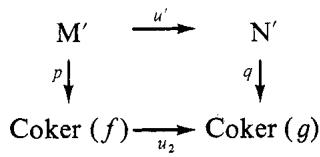
\includegraphics[keepaspectratio]{images/part001_11db974a.jpg}}

Let them be commutative, with i and j denoting the canonical injections, and p and q the canonical surjections.

Indeed, if \(x \in \operatorname{Ker}(f)\) , we have \(f(x) = 0\) and \(g(u(x)) = u'(f(x)) = 0\) , hence \(u(x) \in \operatorname{Ker}(g)\) , and the existence and uniqueness of \(u_1\) are then immediate. Likewise, we have

\[
u ^ {\prime} (f (\mathbf {M})) = g (u (\mathbf {M})) \subset g (\mathbf {N}),
\]

hence \(u'\) gives by passage to quotients a homomorphism

\[
u _ {2}: \operatorname{Coker} (f) \rightarrow \operatorname{Coker} (g),
\]

which is the unique homomorphism for which (9) is commutative.

Now start from a commutative diagram (4) of A-modules; by virtue of Lemma 1 there corresponds to it a commutative diagram

\[
\begin{array}{c c c c c} \operatorname{Ker} (f) \xrightarrow {u _ {1}} & \operatorname{Ker} (g) \xrightarrow {v _ {1}} & \operatorname{Ker} (h) \\ i \Big \downarrow & j \Big \downarrow & k \Big \downarrow \\ \mathbf {M} & u & \mathbf {N} & v & \mathbf {P} \\ f \Big \downarrow & g \Big \downarrow & h \Big \downarrow \\ \mathbf {M} ^ {\prime} & u ^ {\prime} & \mathbf {N} ^ {\prime} & v ^ {\prime} & \mathbf {P} ^ {\prime} \\ p \Big \downarrow & q \Big \downarrow & r \Big \downarrow \\ \operatorname{Coker} (f) \xrightarrow {u _ {2}} & \operatorname{Coker} (g) \xrightarrow {v _ {2}} & \operatorname{Coker} (h) \end{array}\tag{10}
\]

where \(i, j, k\) are the canonical injections, \(p, q, r\) the canonical surjections, \(u_{1}, u_{2}\) (resp. \(v_{1}, v_{2}\) ) the homomorphisms deduced from \(u\) , \(u'\) (resp. \(v, v'\) ) by Lemma 1.

PROPOSITION 2. --- Suppose that in the commutative diagram (4), the sequences \((u, v)\) and \((u', v')\) are exact. Then:

\begin{enumerate}
\def\labelenumi{(\roman{enumi})}
\item
  One has \(v_{1} \circ u_{1} = 0\) ; if \(u'\) is injective, the sequence \((u_{1}, v_{1})\) is exact.
\item
  One has \(v_2 \circ u_2 = 0\) ; if v is surjective, the sequence \((u_2, v_2)\) is exact.
\item
  Suppose \(u'\) injective and \(v\) surjective. There then exists one and only one homomorphism \(d: \operatorname{Ker}(h) \to \operatorname{Coker}(f)\) having the following property: if \(z \in \operatorname{Ker}(h)\) , \(y \in \mathbf{N}\) and \(x' \in \mathbf{M}'\) satisfy the relations \(v(y) = k(z)\) and \(u'(x') = g(y)\) , we have \(d(z) = p(x')\) . Moreover, the sequence
\end{enumerate}

(*) \(\operatorname{Ker}(f) \xrightarrow{u_1} \operatorname{Ker}(g) \xrightarrow{v_1} \operatorname{Ker}(h) \xrightarrow{d} \operatorname{Coker}(f) \xrightarrow{u_2} \operatorname{Coker}(g) \xrightarrow{v_2} \operatorname{Coker}(h)\) is exact.

\pandocbounded{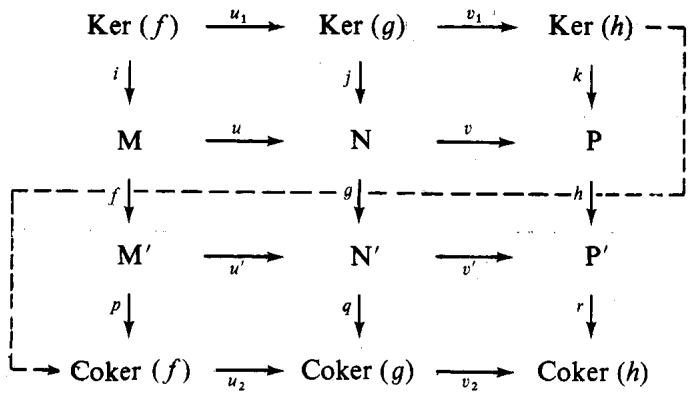
\includegraphics[keepaspectratio]{images/part001_0570902c.jpg}}

Let us prove (i). Since \(u_{1}\) and \(v_{1}\) have the same graphs as the restrictions of \(u\) and \(v\) to \(\operatorname{Ker}(f)\) and \(\operatorname{Ker}(g)\) respectively, we have \(v_{1} \circ u_{1} = 0\) . We have

\[
\operatorname{Ker} \left(v _ {1}\right) = \operatorname{Ker} (g) \cap \operatorname{Ker} (v) = \operatorname{Ker} (g) \cap \operatorname{Im} (u) = \operatorname{Im} (j) \cap \operatorname{Im} (u).
\]

But by prop. 1 (i), we have \(\operatorname{Ker}(v_1) = \operatorname{Im}(j \circ u_1) = \operatorname{Im}(u_1)\) if \(u'\) is injective. Let us prove (ii). Since \(u_2\) and \(v_2\) come from \(u\) and \(v\) by passing to quotients, it is clear that \(v_2 \circ u_2 = 0\) . Suppose \(v\) surjective; since \(q\) and \(p\) are surjective, we have, by virtue of the hypotheses and of prop. 1 (ii)

\[
\begin{array}{r l} \operatorname{Ker} (v _ {2}) & = q (\operatorname{Ker} (v _ {2} \circ q)) = q (\operatorname{Ker} (v ^ {\prime}) + \operatorname{Im} (g)) = q (\operatorname{Ker} (v ^ {\prime})) \\ & = q (\operatorname{Im} (u ^ {\prime})) = \operatorname{Im} (q \circ u ^ {\prime}) = \operatorname{Im} (u _ {2} \circ p) = \operatorname{Im} (u _ {2}). \end{array}
\]

Finally, let us prove (iii). For \(z \in \operatorname{Ker}(h)\) there exists \(y \in \mathbf{N}\) such that \(v(y) = k(z)\) since \(v\) is surjective; moreover, we have \(v'(g(y)) = h(k(z)) = 0\) and consequently there exists a unique \(x' \in \mathbf{M}'\) such that \(u'(x') = g(y)\) since \(u'\) is injective. Let us show that the element \(p(x') \in \operatorname{Coker}(f)\) is independent of the element \(y \in \mathbf{N}\) such that \(v(y) = k(z)\) . Indeed, if \(y_1 \in \mathbf{N}\) is a second element such that \(v(y_1) = k(z)\) , we have \(y_1 = y + u(x)\) where \(x \in \mathbf{M}\) . Let us show that if \(x_1' \in \mathbf{M}'\) is such that \(u'(x_1') = g(y_1)\) , we have \(x_1' = x' + f(x)\) ; indeed, we have \(u'(x' + f(x)) = u'(x') + u'(f(x)) = g(y) + g(u(x)) = g(y + u(x)) = g(y_1)\) . Finally, we conclude that \(p(x_1') = p(x') + p(f(x)) = p(x')\) . We can therefore set \(d(z) = p(x')\) and we have thus defined a map \(d: \operatorname{Ker}(h) \to \operatorname{Coker}(f)\) .

If now \(z_{1}, z_{2}\) are elements of \(\operatorname{Ker}(h)\) , if \(\lambda_{1}, \lambda_{2} \in \mathbf{A}\) and \(z = \lambda_{1} z_{1} + \lambda_{2} z_{2}\) , we take elements \(y_{1}\) and \(y_{2}\) of \(\mathbf{N}\) such that \(v(y_{1}) = k(z_{1})\) and \(v(y_{2}) = k(z_{2})\) and we choose for \(y \in \mathbf{N}\) the element \(\lambda_{1} y_{1} + \lambda_{2} y_{2}\) ; it is then immediate that

\[
d (z) = \lambda_ {1} d (z _ {1}) + \lambda_ {2} d (z _ {2}),
\]

so d is a homomorphism.

Suppose that \(z = v_1(t)\) for a \(t \in \operatorname{Ker}(g)\) ; we will then take for \(y \in \mathbf{N}\) the element \(j(t)\) . Since \(g(j(t)) = 0\) , we conclude \(d(z) = 0\) , hence \(d \circ v_1 = 0\) . Conversely, suppose that \(d(z) = 0\) . With the preceding notation, we therefore have \(x' = f(x)\) , where \(x \in M\) . In this case, we have \(g(y) = u'(f(x)) = g(u(x))\) , or equivalently \(g(y - u(x)) = 0\) . The element \(y - u(x)\) is therefore of the form \(j(n)\) for \(n \in \operatorname{Ker}(g)\) , and we have

\[
k (z) = v (y) = v (u (x) + j (n)) = v (j (n)) = k \left(v _ {1} (n)\right);
\]

since \(k\) is injective, \(z = v_{1}(n)\) , which proves that the sequence (*) is exact at \(\operatorname{Ker}(h)\) . Finally, we have (still with the same notation)

\[
u _ {2} (d (z)) = u _ {2} \left(p \left(x ^ {\prime}\right)\right) = q \left(u ^ {\prime} \left(x ^ {\prime}\right)\right) = q (g (y)) = 0 \quad \text {   hence   } \quad u _ {2} \circ d = 0.
\]

Conversely, suppose that an element \(w = p(x')\) of Coker \((f)\) is such that

\[
u _ {2} (w) = u _ {2} \left(p \left(x ^ {\prime}\right)\right) = 0 \quad \left(\operatorname{with} x ^ {\prime} \in \mathbf {M} ^ {\prime}\right).
\]

We therefore have \(q(u'(x')) = 0\) , and consequently \(u'(x') = g(y)\) for a \(y \in \mathbb{N}\) ; since \(v'(u'(x')) = 0\) , we have \(v'(g(y)) = 0\) , hence \(h(v(y)) = 0\) , in other words \(v(y) = k(z)\) for a \(z \in \operatorname{Ker}(h)\) , and by definition \(w = d(z)\) , which shows that the sequence (*) is exact at Coker ( \(f\) ). We saw in (i) that it is exact at Ker ( \(g\) ) and in (ii) that it is exact at Coker ( \(g\) ), which completes the proof of (iii).

COROLLARY 1. --- Suppose that diagram (4) is commutative and has exact rows. Then:

\begin{enumerate}
\def\labelenumi{(\roman{enumi})}
\item
  If \(u'\) , \(f\) and \(h\) are injective, \(g\) is injective.
\item
  If v, f, and h are surjective, then g is surjective.
\end{enumerate}

Assertion (i) follows from assertion (i) of prop. 2: indeed, we have \(\operatorname{Ker}(f) = 0\) and \(\operatorname{Ker}(h) = 0\) , hence \(\operatorname{Ker}(g) = 0\) .

Assertion (ii) follows from assertion (ii) of prop. 2: indeed, we have Coker \(f\) = 0 and Coker \(h\) = 0, hence Coker \(g\) = 0.

COROLLARY 2. --- Suppose that diagram (4) is commutative and has exact rows. Under these conditions:

\begin{enumerate}
\def\labelenumi{(\roman{enumi})}
\item
  If g is injective and if f and v are surjective, then h is injective.
\item
  If g is surjective and if h and u' are injective, then f is surjective.
\end{enumerate}

To prove (i), consider the diagram

\[
\begin{array}{c c c c c} u (\mathbf {M}) & \xrightarrow {w} & \mathbf {N} & \xrightarrow {v} & \mathbf {P} \\ f ^ {\prime} \Big \downarrow & & g \Big \downarrow & & h \Big \downarrow \\ u ^ {\prime} (\mathbf {M} ^ {\prime}) & \xrightarrow {w ^ {\prime}} & \mathbf {N} ^ {\prime} & \xrightarrow {v ^ {\prime}} & \mathbf {P} ^ {\prime} \end{array}
\]

where \(f'\) is the map having the same graph as the restriction of \(g\) to \(u(\mathbf{M})\) , \(w\) and \(w'\) the canonical injections; it is clear that this diagram is commutative and has exact rows. Moreover \(w'\) is injective, and by hypothesis \(v\) is surjective; hence by prop. 2 (iii) we have an exact sequence

\[
\operatorname{Ker} (g) \longrightarrow \operatorname{Ker} (h) \xrightarrow {d} \operatorname{Coker} \left(f ^ {\prime}\right);
\]

since g is injective and \(f'\) is surjective, we therefore have Ker (h) = 0.

To prove (ii), consider the diagram

\[
\begin{array}{c c c c c} \mathbf {M} & \stackrel {{u}} {{\longrightarrow}} & \mathbf {N} & \stackrel {{w}} {{\longrightarrow}} & v (\mathbf {N}) \\ f \Big \downarrow & & g \Big \downarrow & & h ^ {\prime} \Big \downarrow \\ \mathbf {M} ^ {\prime} & \stackrel {{u ^ {\prime}}} {{\longrightarrow}} & \mathbf {N} ^ {\prime} & \stackrel {{w ^ {\prime}}} {{\longrightarrow}} & v ^ {\prime} (\mathbf {N} ^ {\prime}) \end{array}
\]

where this time \(h'\) is the map having the same graph as the restriction of \(h\) to \(v(\mathbf{N})\) , and \(w\) and \(w'\) have respectively the same graphs as \(v\) and \(v'\) ; this diagram is commutative and its rows are exact. Moreover \(w\) is surjective and by hypothesis \(u'\) is injective; hence by prop. 2 (iii) we have an exact sequence

\[
\operatorname{Ker} \left(h ^ {\prime}\right) \xrightarrow {d} \operatorname{Coker} (f) \longrightarrow \operatorname{Coker} (g);
\]

since \(g\) is surjective and \(h'\) is injective, we therefore have Coker \((f) = 0\) .

COROLLARY 3 (Five lemma). --- Consider a commutative diagram of A-modules

\[
\begin{array}{c c c c c c c c c} \mathbf {M} _ {1} & \xrightarrow {u _ {1}} & \mathbf {M} _ {2} & \xrightarrow {u _ {2}} & \mathbf {M} _ {3} & \xrightarrow {u _ {3}} & \mathbf {M} _ {4} & \xrightarrow {u _ {4}} & \mathbf {M} _ {5} \\ f _ {1} \Big \downarrow & & f _ {2} \Big \downarrow & & f _ {3} \Big \downarrow & & f _ {4} \Big \downarrow & & f _ {5} \Big \downarrow \\ \mathbf {M} _ {1} ^ {\prime} & \xrightarrow {u _ {1} ^ {\prime}} & \mathbf {M} _ {2} ^ {\prime} & \xrightarrow {u _ {2} ^ {\prime}} & \mathbf {M} _ {3} ^ {\prime} & \xrightarrow {u _ {3} ^ {\prime}} & \mathbf {M} _ {4} ^ {\prime} & \xrightarrow {u _ {4} ^ {\prime}} & \mathbf {M} _ {5} ^ {\prime} \end{array}
\]

where the rows are exact.

\begin{enumerate}
\def\labelenumi{(\roman{enumi})}
\item
  If \(f_{2}\) and \(f_{4}\) are injective and \(f_{1}\) surjective, \(f_{3}\) is injective.
\item
  If \(f_{2}\) and \(f_{4}\) are surjective and \(f_{5}\) injective, \(f_{3}\) is surjective.
\end{enumerate}

In particular, if \(f_1, f_2, f_4\) and \(f_5\) are isomorphisms, then so is \(f_3\) . To prove (i), set \(\tilde{\mathbf{M}}_2 = \text{Coker } (u_1), \tilde{\mathbf{M}}_2' = \text{Coker } (u_1')\) and let us denote by \(\tilde{f}_2: \tilde{\mathbf{M}}_2 \to \tilde{\mathbf{M}}_2'\) the map deduced from \(f_2\) . It follows from cor. 2 (i) that \(\tilde{f}_2\) is injective. Applying cor. 1 (i) to the diagram

\[
\begin{array}{c c c c c} \tilde {\mathbf {M}} _ {2} & \xrightarrow {\tilde {u} _ {2}} & \mathbf {M} _ {3} & \xrightarrow {u _ {3}} & \mathbf {M} _ {4} \\ \tilde {f} _ {2} \Big \downarrow & & f _ {3} \Big \downarrow & & f _ {4} \Big \downarrow \\ \tilde {\mathbf {M}} _ {2} ^ {\prime} & \xrightarrow {\tilde {u} _ {2} ^ {\prime}} & \mathbf {M} _ {3} ^ {\prime} & \xrightarrow {u _ {3} ^ {\prime}} & \mathbf {M} _ {4} ^ {\prime} \end{array}
\]

where \(\tilde{u}_2\) and \(\tilde{u}_2'\) are deduced from \(u_2\) and \(u_2'\) , we see that \(f_3\) is injective.

To prove (ii), set \(\tilde{\mathbf{M}}_{4} = \operatorname{Ker}(u_{4}), \tilde{\mathbf{M}}_{4}' = \operatorname{Ker}(u_{4}')\) and let us denote by \(\tilde{f}_{4}: \tilde{\mathbf{M}}_{4} \to \tilde{\mathbf{M}}_{4}'\) the map induced by \(f_{4}\) . It follows from cor. 2 (ii) that \(\tilde{f}_{4}\) is surjective. Applying cor. 1 (ii) to the diagram

\[
\begin{array}{c c c c c} \mathbf {M} _ {2} & \xrightarrow {u _ {2}} & \mathbf {M} _ {3} & \xrightarrow {\tilde {u} _ {3}} & \tilde {\mathbf {M}} _ {4} \\ f _ {2} \Big \downarrow & & f _ {3} \Big \downarrow & & \tilde {f} _ {4} \Big \downarrow \\ \mathbf {M} _ {2} ^ {\prime} & \xrightarrow {u _ {2} ^ {\prime}} & \mathbf {M} _ {3} ^ {\prime} & \xrightarrow {\tilde {u} _ {3} ^ {\prime}} & \tilde {\mathbf {M}} _ {4} ^ {\prime} \end{array}
\]

where \(\tilde{u}_3\) and \(\tilde{u}_3'\) have the same graph as \(u_3\) and \(u_3'\) , we see that \(f_3\) is surjective.

\subsection{Flat modules}

DEFINITION 1. --- The A-module E is said to be flat if, for every exact sequence of right A-modules and homomorphisms

\[
\mathbf {M} ^ {\prime} \xrightarrow {u} \mathbf {M} \xrightarrow {v} \mathbf {M} ^ {\prime \prime},\tag{11}
\]

the sequence of Z-linear maps

\[
\mathbf {M} ^ {\prime} \otimes_ {\mathbf {A}} \mathrm{E} \xrightarrow {u \otimes 1} \mathbf {M} \otimes_ {\mathbf {A}} \mathrm{E} \xrightarrow {v \otimes 1} \mathbf {M} ^ {\prime \prime} \otimes_ {\mathbf {A}} \mathrm{E}\tag{12}
\]

is exact.

PROPOSITION 3. --- For the A-module E to be flat, it is necessary and sufficient that, for every injective A-homomorphism \(u: \mathbf{M}' \to \mathbf{M}\) of right A-modules, the map \(u \otimes 1: \mathbf{M}' \otimes_{\mathbf{A}} \mathbf{E} \to \mathbf{M} \otimes_{\mathbf{A}} \mathbf{E}\) be injective.

If E is flat and \(u: \mathbf{M}' \to \mathbf{M}\) injective, the sequence \(0 \longrightarrow \mathbf{M}' \stackrel{u}{\longrightarrow} \mathbf{M}\) is exact, hence also

the sequence 0 \(\longrightarrow\) M' \(\otimes_{\mathbf{A}}\) E \(\xrightarrow{u\otimes1}\) M \(\otimes_{\mathbf{A}}\) E, and \(u\otimes1\) is injective. Conversely, consider the exact sequence (11); set M'\,' \(_{1}\) = v(M), and let i : M'\,' \(_{1}\) → M'\,' be the canonical injection

and \(p:\mathbf{M}\to\mathbf{M}_{1}^{\prime\prime}\) the map \(m\mapsto v(m)\) . The sequence \(\mathbf{M}^{\prime}\xrightarrow{u}\mathbf{M}\xrightarrow{p}\mathbf{M}_{1}^{\prime\prime}\longrightarrow0\)

is exact; by II, p.~58, prop. 5, the sequence \(\mathbf{M}' \otimes_{\mathbf{A}} \mathbf{E} \xrightarrow{u \otimes 1} \mathbf{M} \otimes_{\mathbf{A}} \mathbf{E} \xrightarrow{p \otimes 1} \mathbf{M}_{1}'' \otimes_{\mathbf{A}} \mathbf{E}\) is therefore exact. Moreover, we have \(v = i \circ p\) , hence \((v \otimes 1) = (i \otimes 1) \circ (p \otimes 1)\) ; if E satisfies the condition of the statement, then \(i \otimes 1\) is injective, therefore

\[
\operatorname{Ker} (v \otimes 1) = \operatorname{Ker} (p \otimes 1) = \operatorname{Im} (u \otimes 1)
\]

and the sequence (12) is exact.

PROPOSITION 4. ---(i) Let \((\mathbf{E}_i)_{i\in \mathbf{I}}\) be a family of A-modules, \(\mathrm{E} = \bigoplus_{i\in \mathbf{I}}\mathrm{E}_i\) their direct sum

For the A-module E to be flat, it is necessary and sufficient that each of the \(E_{i}\) be so.

\begin{enumerate}
\def\labelenumi{(\roman{enumi})}
\setcounter{enumi}{1}
\tightlist
\item
  Let I be a right-filtered preordered set, \((\mathrm{E}_{\alpha}, f_{\beta\alpha})\) an inductive system of A-modules relative to I, \(E = \varinjlim E_{\alpha}\) its inductive limit. If each of the A-modules \(E_{\alpha}\) is flat, then E is flat.
\end{enumerate}

Let \(M^{\prime} \rightarrow M \rightarrow M^{\prime\prime}\) be an exact sequence of right A-modules.

\begin{enumerate}
\def\labelenumi{(\roman{enumi})}
\item
  For the sequence \(\bigoplus_{i\in I}(\mathbf{M}^{\prime}\otimes_{\mathbf{A}}\mathbf{E}_{i})\to \bigoplus_{i\in I}(\mathbf{M}\otimes_{\mathbf{A}}\mathbf{E}_{i})\to \bigoplus_{i\in I}(\mathbf{M}^{\prime \prime}\otimes_{\mathbf{A}}\mathbf{E}_{i})\) to be exact, it is necessary and sufficient that each of the sequences \(\mathbf{M}^{\prime}\otimes_{\mathbf{A}}\mathbf{E}_{i}\to \mathbf{M}\otimes_{\mathbf{A}}\mathbf{E}_{i}\to \mathbf{M}^{\prime \prime}\otimes_{\mathbf{A}}\mathbf{E}_{i}\) be exact (II, p.~13, prop. 7), which proves (i) since \(\oplus (\mathbf{M}\otimes_{\mathbf{A}}\mathbf{E}_{i})\) is canonically identified with \(\mathbf{M}\otimes_{\mathbf{A}}\mathbf{E}\) (II, p.~61, prop. 7).
\item
  By hypothesis, each of the sequences \(\mathbf{M}' \otimes_{\mathbf{A}} \mathbf{E}_i \to \mathbf{M} \otimes_{\mathbf{A}} \mathbf{E}_i \to \dot{\mathbf{M}}'' \otimes_{\mathbf{A}} \mathbf{E}_i\) is exact, hence so is the sequence \(\mathbf{M}' \otimes_{\mathbf{A}} \mathbf{E} \to \mathbf{M} \otimes_{\mathbf{A}} \mathbf{E} \to \mathbf{M}'' \otimes_{\mathbf{A}} \mathbf{E}\) , since passage to the inductive limit commutes with tensor product (II, p.~93, prop. 7) and preserves exactness (II, p.~91, prop. 3).
\end{enumerate}

Examples. --- 1) It is clear that \(A_{s}\) is a flat A-module; it then follows from prop. 4 (i) that every free A-module, and more generally every projective A-module, is flat (see also II, p.~63, cor. 6).

* Conversely, every flat A-module of finite presentation is projective (no. 5). *

\begin{enumerate}
\def\labelenumi{\arabic{enumi})}
\setcounter{enumi}{1}
\item
  By prop. 4 (ii), every A-module which is the inductive limit of a filtered inductive system of free A-modules is flat. We shall prove a converse in no. 6.
\item
  If A is semisimple, every A-module is projective (VIII, § 5, no. 1, prop. 1), hence flat.
\item
  * If A is an artinian local ring (not necessarily commutative), an A-module is flat if and only if it is free (AC II, § 3, no. 2, cor. 2 of prop. 5). *
\item
  If A is an integral domain, the field of fractions K of A is a flat A-module (II, p.~118, prop. 27).
\item
  * In AC II and III, we shall study two important examples of flat A-modules when A is commutative: the rings of fractions \(S^{-1}\) A, and when A is noetherian, the separated completions of A for the J-adic topologies. *
\item
  Let \(a \in \mathbf{A}\) such that the map \(a_{\mathbf{A}}: x \mapsto ax\) of \(\mathbf{A}\) to \(\mathbf{A}\) is injective (“ \(a\) is not a left zero-divisor”). If \(\mathbf{E}\) is a flat \(\mathbf{A}\) -module, then the homothety \(a_{\mathbf{E}}\) is injective, since it is identified with \(a_{\mathbf{A}} \otimes 1: \mathbf{A}_{d} \otimes_{\mathbf{A}} \mathbf{E} \to \mathbf{A}_{d} \otimes_{\mathbf{A}} \mathbf{E}\) . In particular, if \(\mathbf{A}\) is an integral domain, every flat \(\mathbf{A}\) -module is torsion-free. Conversely, if \(\mathbf{A}\) is principal, every torsion-free \(\mathbf{A}\) -module is flat: indeed, if the \(\mathbf{A}\) -module \(\mathbf{E}\) is torsion-free, every finitely generated submodule of \(\mathbf{E}\) is free (VII, § 4, no. 4, cor. 2 to th. 4), and \(\mathbf{E}\) is a filtering increasing union of flat submodules, hence is flat (prop. 4 (ii)).
\item
  Let B be a ring and \(\rho: \mathbf{A} \to \mathbf{B}\) a homomorphism. If E is a flat A-module, the B-module \(\mathbf{E}_{(\mathbf{B})} = \mathbf{B} \otimes_{\mathbf{A}} \mathbf{E}\) is flat. Indeed, let \(u: \mathbf{N}' \to \mathbf{N}\) be an injective homomorphism of right B-modules; then \(u \otimes_{\mathbf{B}} 1_{\mathbf{E}_{(\mathbf{B})}}\) is canonically identified with the homomorphism \(u \otimes_{\mathbf{A}} 1_{\mathbf{E}}: \mathbf{N}' \otimes_{\mathbf{A}} \mathbf{E} \to \mathbf{N} \otimes_{\mathbf{A}} \mathbf{E}\) , which is injective if E is flat.
\item
  Suppose that \(\mathbf{A} = \mathbf{K}[\mathbf{X}, \mathbf{Y}]\) , where \(\mathbf{K}\) is a field. Then the maximal ideal \(m\) generated by \(\mathbf{X}\) and \(\mathbf{Y}\) is a torsion-free A-module, but not flat. Indeed, consider the ring \(\mathbf{B} = \mathbf{A}/(\mathbf{Y})\) , which is isomorphic to \(\mathbf{K}[\mathbf{X}]\) , hence an integral domain. The B-module \(m_{(B)}\) is isomorphic to \(m/Ym = (X, Y)/(XY, Y^2)\) , in which the class of \(Y\) is torsion. Consequently, \(m_{(B)}\) is not a flat B-module, hence \(m\) is not flat.
\item
  Suppose A is commutative. Let B be the algebra \(\mathbf{A}[\mathbf{X}_1, \ldots, \mathbf{X}_n] / (\mathbf{P})\) , where P is a nonzero polynomial. For every prime ideal p of A, denote by \(\kappa(p)\) the field of fractions of the integral domain \(\mathbf{A} / p\) , \(\mathbf{E}(p)\) the algebra \(\kappa(p) [\mathbf{X}_1, \ldots, \mathbf{X}_n]\) and \(\mathbf{P}(p)\) the image of P in \(\mathbf{E}(p)\) under the canonical mapping.
\end{enumerate}

One can show that, for B to be a flat A-module, it suffices that \(P(p) \neq 0\) for every prime ideal p of A. If A is an integral domain, this condition is necessary.

* In geometric language, consider the projection \(\pi: \text{Spec}(B) \to \text{Spec}(A)\) . For every \(p \in \text{Spec}(A)\) the fiber \(\pi^{-1}(p)\) is identified with the subvariety \(V_p\) of the affine space \(\mathbf{A}_{\kappa(p)}^n = \text{Spec}(E(p))\) defined by \(P(p)\) , and the set \(F\) of \(p\) for which this subvariety is the entire space (i.e.~for which \(P(p) = 0\) ) is a closed subset of

Spec(A). The preceding condition means that this closed set is empty, in other words that for every p the subvariety \(V_{p}\) is a hypersurface in \(\mathbf{A}_{\kappa(p)}^{n}\) . *

\begin{enumerate}
\def\labelenumi{\arabic{enumi})}
\setcounter{enumi}{10}
\tightlist
\item
  Let S and X be two complex analytic spaces, and \(f: \mathbf{X} \to \mathbf{S}\) a morphism. We say that \(f\) is flat at a point \(x\) of \(\mathbf{X}\) if \(\mathcal{O}_{\mathbf{X},x}\) , considered as \(\mathcal{O}_{\mathbf{S},f(x)}\) -module by means of the homomorphism \(f^{*}: \mathcal{O}_{\mathbf{S},f(x)} \to \mathcal{O}_{\mathbf{X},x}\) , is flat. The set of points of \(\mathbf{X}\) where \(f\) is flat is an open subset of \(\mathbf{X}\) , and the restriction of \(f\) to this open set is an open map. If \(\mathbf{X}\) and \(\mathbf{S}\) are connected finite-dimensional analytic manifolds, \(f\) is flat (at every point of \(\mathbf{X}\) ) if and only if \(f(\mathbf{X})\) is open in \(\mathbf{S}\) and the fibers \(f^{-1}(s)\) , for \(s \in f(\mathbf{X})\) all have the same dimension. *
\end{enumerate}

\subsection{Modules of finite presentation}

A presentation (or presentation of length 1) of an A-module E is an exact sequence

\[
\mathrm{L} _ {1} \rightarrow \mathrm{L} _ {0} \rightarrow \mathrm{E} \rightarrow 0\tag{13}
\]

of A-modules where \(\mathbf{L}_0\) and \(\mathbf{L}_1\) are free.

Every A-module E admits a presentation. Indeed, we know (II, p.~27, prop. 20) that there exists a surjective homomorphism \(u: \mathbf{L}_0 \to \mathbf{E}\) , where \(\mathbf{L}_0\) is free; if R is the kernel of \(u\) , there likewise exists a surjective homomorphism \(v: \mathbf{L}_1 \to \mathbf{R}\) where \(\mathbf{L}_1\) is free. If one regards \(v\) as a homomorphism of \(\mathbf{L}_1\) to \(\mathbf{L}_0\) , the sequence \(\mathbf{L}_1 \xrightarrow{v} \mathbf{L}_0 \xrightarrow{u} \mathbf{E} \longrightarrow 0\) is exact by definition, whence our assertion.

If \(\rho: A \to B\) is a ring homomorphism, every presentation (13) of \(E\) furnishes a presentation of \(E_{(B)} = B \otimes_A E\) :

\[
\mathbf {B} \otimes_ {\mathbf {A}} \mathrm{L} _ {1} \rightarrow \mathbf {B} \otimes_ {\mathbf {A}} \mathrm{L} _ {0} \rightarrow \mathbf {B} \otimes_ {\mathbf {A}} \mathrm{E} \rightarrow 0\tag{14}
\]

by virtue of II, p.~58, prop. 5 and of the fact that \(\mathbf{B} \otimes_{\mathbf{A}} \mathbf{L}\) is a free B-module when L is free.

One says that a presentation (13) of a module E is finite if the free modules \(L_{0}\) and \(L_{1}\) have finite bases. It is clear that if the presentation (13) is finite, so is the presentation (14). One says that E is an A-module of finite presentation if it admits a finite presentation.

PROPOSITION 5. --- (i) Every module admitting a finite presentation is finitely generated.

\begin{enumerate}
\def\labelenumi{(\roman{enumi})}
\setcounter{enumi}{1}
\item
  If A is a left Noetherian ring, every finitely generated A-module admits a finite presentation.
\item
  Every finitely generated projective module admits a finite presentation.
\end{enumerate}

Assertion (i) follows trivially from the definitions. Suppose A is left Noetherian and E is finitely generated. There then exists a surjective homomorphism \(u: L_0 \to E\) , where \(L_0\) is a free A-module having a finite basis; the kernel R of \(u\) is finitely generated, hence there is a surjective homomorphism \(v: L_1 \to R\) where \(L_1\) is free with finite basis, and the exact sequence \(L_1 \xrightarrow{v} L_0 \xrightarrow{u} E \longrightarrow 0\) is a finite presentation of E; whence (ii).

Finally, suppose that E is a finitely generated projective module; it is then a direct summand of a finitely generated free module \(L_{0}\) (II, p.~40, cor. 1); the kernel R of the surjective homomorphism \(L_{0} \rightarrow E\) is then isomorphic to a quotient of \(L_{0}\) , hence is finitely generated, and one finishes as above.

PROPOSITION 6. --- Let A be a ring, E an A-module of finite presentation. For every exact sequence

\[
0 \longrightarrow \mathrm{F} \stackrel {j} {\longrightarrow} \mathrm{G} \stackrel {p} {\longrightarrow} \mathrm{E} \longrightarrow 0
\]

where G is finitely generated, the module F is finitely generated.

Let \(L_{1} \xrightarrow{r} L_{0} \xrightarrow{s} E \longrightarrow 0\) be a finite presentation; if \((e_{i})\) is a basis of \(L_{0}\) , there exists for each i an element \(g_{i} \in G\) such that \(p(g_{i}) = s(e_{i})\) ; the homomorphism \(u : L_{0} \to G\) such that \(u(e_{i}) = g_{i}\) for all i is therefore such that \(s = p \circ u\) . Since \(s \circ r = 0\) , we have \(u(r(L_{1})) \subset \operatorname{Ker} p\) , and since Ker p is isomorphic to F, we see that there is a homomorphism \(v : L_{1} \to F\) such that the diagram

\[
\begin{array}{c c c c c c c} L _ {1} & \xrightarrow {r} & L _ {0} & \xrightarrow {s} & E & \longrightarrow & 0 \\ v \Big \downarrow & & u \Big \downarrow & & ^ {1 _ {E}} \Big \downarrow \\ F & \xrightarrow {} _ {j} & G & \xrightarrow {} _ {p} & E & \longrightarrow & 0 \end{array}
\]

is commutative. Since j is injective and s surjective, one can apply Proposition 2 of X, p.~4, in other words there is an exact sequence

\[
\operatorname{Ker} 1 _ {\mathrm{E}} \xrightarrow {d} \text { Coker } v \longrightarrow \text { Coker } u \longrightarrow \text { Coker } 1 _ {\mathrm{E}}.
\]

This shows that Coker v is isomorphic to \(\mathrm{G}/u(\mathrm{L}_{0})\) , which is finitely generated by hypothesis. Moreover, we have the exact sequence

\[
0 \rightarrow v (\mathbf {L} _ {1}) \rightarrow \mathrm{F} \rightarrow \text { Coker } v \rightarrow 0
\]

and since \(v(\mathbf{L}_1)\) and Coker \(v\) are finitely generated, so is F (II, p.~17, cor. 5).

PROPOSITION 7. --- Let M be an A-module. There exists a right-filtered ordered set I and an inductive system of finitely presented A-modules (M \(_{\alpha}\) , φ \(_{\beta\alpha}\) ) relative to I such that M is isomorphic to lim M \(_{\alpha}\) . If M possesses a generating family of n elements, one may assume that the same is true of the M \(_{\alpha}\) .

Consider a presentation

\[
\mathrm{A} _ {s} ^ {(\mathrm{K})} \xrightarrow {u} \mathrm{A} _ {s} ^ {(\mathrm{L})} \xrightarrow {v} \mathrm{M} \longrightarrow 0;
\]

let I be the set of pairs \(\alpha = (\mathbf{K}', \mathbf{L}')\) , where \(\mathbf{K}'\) (resp. \(\mathbf{L}'\) ) is a finite subset of \(\mathbf{K}\) (resp. L), such that \(u\) induces a map \(u_{\alpha}\) of the submodule \(\mathbf{A}_s^{\mathbf{K}'}\) of \(\mathbf{A}_s^{(\mathbf{K})}\) in the submodule \(\mathbf{A}_s^{\mathbf{L}'}\) of \(\mathbf{A}_s^{(\mathbf{L})}\) ; for \(\alpha \in \mathbf{I}\) , let \(\mathbf{M}_{\alpha}\) be the cokernel of \(u_{\alpha}\) and \(v_{\alpha}: \mathbf{A}_s^{\mathbf{L}'} \to \mathbf{M}_{\alpha}\) the canonical map, so that we have a commutative diagram with exact rows:

\[
\mathrm{A} _ {s} ^ {(\mathrm{K})} \xrightarrow {u} \mathrm{A} _ {s} ^ {(\mathrm{L})} \xrightarrow {i} \mathrm{M} \longrightarrow 0
\]

\[
i _ {\alpha} \uparrow , \quad j _ {\alpha} \uparrow , \quad f _ {\alpha} \uparrow
\]

\[
\mathrm{A} _ {s} ^ {\mathrm{K} ^ {\prime}} \xrightarrow {u _ {\alpha}} \mathrm{A} _ {s} ^ {\mathrm{L} ^ {\prime}} \xrightarrow {v _ {\alpha}} \mathrm{M} _ {\alpha} \longrightarrow 0,
\]

where \(i_{\alpha}\) and \(j_{\alpha}\) are the canonical injections, and where \(f_{\alpha}\) is deduced from \(j_{\alpha}\) by passing to quotients. Order the set I by the relation

\[
\alpha = \left(\mathrm{K} ^ {\prime}, \mathrm{L} ^ {\prime}\right) \leqslant \beta = \left(\mathrm{K} ^ {\prime \prime}, \mathrm{L} ^ {\prime \prime}\right) \quad \text { if } \quad \mathrm{K} ^ {\prime} \subset \mathrm{K} ^ {\prime \prime}, \quad \mathrm{L} ^ {\prime} \subset \mathrm{L} ^ {\prime \prime};
\]

for \(\alpha \leqslant \beta\) , let \(\varphi_{\beta \alpha}: \mathbf{M}_{\alpha} \to \mathbf{M}_{\beta}\) be the homomorphism deduced by passing to quotients from the inclusion of \(\mathbf{A}_s^{L'}\) to \(\mathbf{A}_s^{L''}\) . One then immediately verifies that the ordered set I is filtered, and that \((\mathbf{M}_{\alpha}, \varphi_{\beta \alpha})\) is an inductive system of A-modules and that \((\varphi_{\alpha})\) is an inductive system of A-homomorphisms. Passing to the inductive limit, one obtains a commutative diagram

\[
\begin{array}{c c c c c} \mathbf {A} _ {s} ^ {(\mathbf {K})} & \stackrel {{u}} {{\longrightarrow}} & \mathbf {A} _ {s} ^ {(L)} & \stackrel {{v}} {{\longrightarrow}} & \mathbf {M} \\ i \uparrow & & j \uparrow & & \varphi \uparrow \\ \underline {{\lim}} \mathbf {A} _ {s} ^ {\mathbf {K} ^ {\prime}} & \longrightarrow & \underline {{\lim}} \mathbf {A} _ {s} ^ {\mathbf {L} ^ {\prime}} & \longrightarrow & \underline {{\lim}} \mathbf {M} _ {\alpha} \longrightarrow 0; \end{array}\tag{15}
\]

The rows of this diagram are exact (II, p.~91, prop. 3); since i and j are bijective, φ is also bijective (X, p.~7, cor. 3), whence the proposition.

\subsection{Homomorphisms of a finitely presented module}

Let E be an A-module. If I is a filtered preordered set and \((\mathbf{G}_{i}, u_{ji})\) an inductive system of A-modules relative to I, the canonical maps \(G_{i} \to \varinjlim G_{i}\) induce homomorphisms \(\operatorname{Hom}_{\mathbf{A}}(\mathbf{E}, \mathbf{G}_{i}) \to \operatorname{Hom}_{\mathbf{A}}(\mathbf{E}, \varinjlim \mathbf{G}_{i})\) whence a homomorphism said to be canonical

\[
\varinjlim_ {i \in \mathrm{I}} \operatorname{Hom} _ {\mathrm{A}} (\mathrm{E}, \mathrm{G} _ {i}) \rightarrow \operatorname{Hom} _ {\mathrm{A}} (\mathrm{E}, \varinjlim_ {i \in \mathrm{I}} \mathrm{G} _ {i}).\tag{16}
\]

Let B be another ring, F a B-module, G an (A, B)-bimodule; we defined in II, p.~75 a canonical homomorphism:

\[
\operatorname{Hom} _ {\mathbf {A}} (\mathrm{E}, \mathrm{G}) \otimes_ {\mathbf {B}} \mathrm{F} \rightarrow \operatorname{Hom} _ {\mathbf {A}} (\mathrm{E}, \mathrm{G} \otimes_ {\mathbf {B}} \mathrm{F}).\tag{17}
\]

PROPOSITION 8. --- a) If the A-module E is finitely generated (resp. finitely presented), the canonical homomorphism (16) is injective (resp. bijective).

\begin{enumerate}
\def\labelenumi{\alph{enumi})}
\setcounter{enumi}{1}
\tightlist
\item
  Suppose that the B-module F is flat; if the A-module E is finitely generated (resp. finitely presented), the canonical homomorphism (17) is injective (resp. bijective). Let us prove, for example, b), the proof of a) being analogous. Consider A, B, F, G as fixed, and, for every right A-module E, set
\end{enumerate}

\[
\mathrm{T} (\mathrm{E}) = \operatorname{Hom} _ {\mathrm{A}} (\mathrm{E}, \mathrm{G}) \otimes_ {\mathrm{B}} \mathrm{F}, \quad \mathrm{T} ^ {\prime} (\mathrm{E}) = \operatorname{Hom} _ {\mathrm{A}} (\mathrm{E}, \mathrm{G} \otimes_ {\mathrm{B}} \mathrm{F})
\]

and let us denote by \(\nu_{\mathbf{E}}\) the homomorphism (17); for every homomorphism \(v: \mathbf{E} \to \mathbf{E}'\) of right A-modules, set \(\mathbf{T}(v) = \operatorname{Hom}(v, 1_{\mathbf{G}}) \otimes 1_{\mathbf{F}}\) and \(\mathbf{T}'(v) = \operatorname{Hom}(v, 1_{\mathbf{G}} \otimes 1_{\mathbf{F}})\) .

Let \(L_{1} \xrightarrow{v} L_{0} \xrightarrow{w} E \to 0\) be a presentation of E; we assume the free module \(L_{0}\) (resp. the free modules \(L_{0}\) and \(L_{1}\) ) to be finitely generated. The diagram

\[
\begin{array}{c} 0 \to \mathrm{T(E)} \xrightarrow {\mathrm{T(w)}} \mathrm {T(L_ {0})} \xrightarrow {\mathrm{T(v)}} \mathrm {T(L_ {1})} \\ v _ {\mathrm{E}} \Big \downarrow \qquad \qquad \qquad \qquad \qquad \qquad \qquad \qquad \qquad \qquad \qquad \qquad \qquad \qquad \qquad \qquad \qquad \qquad \qquad \qquad \qquad \qquad \qquad \qquad \qquad \qquad \qquad \qquad \qquad \qquad \qquad \qquad \qquad \qquad 0 \to \mathrm {T^ {\prime} (E)} \xrightarrow [ \mathrm {T^ {\prime} (w)} ]{} \mathrm {T^ {\prime} (L_ {0})} \xrightarrow [ \mathrm {T^ {\prime} (v)} ]{} \mathrm {T^ {\prime} (L_ {1})} \end{array}\tag{18}
\]

is commutative, and its second row is exact (II, p.~36, th. 1); moreover, the sequence

\[
0 \rightarrow \operatorname{Hom} _ {\mathbf {A}} (\mathrm{E}, \mathrm{G}) \rightarrow \operatorname{Hom} _ {\mathbf {A}} (\mathrm{L} _ {0}, \mathrm{G}) \rightarrow \operatorname{Hom} _ {\mathbf {A}} (\mathrm{L} _ {1}, \mathrm{G})
\]

is exact (loc. cit.), and since F is flat, the first row of (18) is also an exact sequence (X, p.~8, def. 1). That being so, we know that \(v_{L_0}\) is bijective (resp. that \(v_{L_0}\) and \(v_{L_1}\) are bijective) (II, p.~75, prop. 2). If one assumes only \(v_{L_0}\) bijective, it follows from (18) that \(v_{L_0} \circ T(w) = T'(w) \circ v_E\) is injective, therefore \(v_E\) is also. If we suppose that \(v_{L_0}\) and \(v_{L_1}\) both are bijective, we deduce from Cor. 2 (ii) of X, p.~6 that \(v_E\) is surjective, and since we have just seen that \(v_E\) is injective, it is bijective.

COROLLARY. --- Every flat module of finite presentation is projective.

Indeed, let E be a flat A-module of finite presentation. Applying (b) to the case \(\mathbf{B} = \mathbf{A}\) , \(\mathbf{G} = {}_{\mathrm{s}}\mathbf{A}_{\mathrm{d}}\) , \(\mathbf{F} = \mathbf{E}\) , we see that the canonical homomorphism

\[
\operatorname{Hom} _ {\mathbf {A}} (\mathbf {E}, \mathbf {A}) \otimes_ {\mathbf {A}} \mathbf {E} \rightarrow \operatorname{Hom} _ {\mathbf {A}} (\mathbf {E}, \mathbf {E})
\]

is surjective. This implies that E is projective (II, p.~77, Remark 1).

By the preceding corollary and Prop. 5 of X, p.~10, there is an identity between finitely presented flat modules and finitely generated projective modules. On the other hand, there exist finitely generated flat modules that are not finitely presented, hence not projective (cf.~X, p.~170, Exercise 17; see however X, p.~169, Exercises 13 and 14).

\subsection{Structure of flat modules}

Lemma 2. --- Let I be a right-filtered ordered set, \((\mathrm{E}_{\alpha}, \varphi_{\beta\alpha})\) an inductive system of sets relative to I, E its inductive limit, and \(\varphi_{\alpha}: E_{\alpha} \to E\) , \(\alpha \in I\) , the canonical maps. Let \(f: I \to I\) be a map such that \(f(\alpha) > \alpha\) for \(\alpha \in I\) , and suppose given, for each \(\alpha \in I\) , a set \(L_{\alpha}\) and maps \(u_{\alpha}: E_{\alpha} \to L_{\alpha}\) and \(v_{\alpha}: L_{\alpha} \to E_{f(\alpha)}\) such that \(v_{\alpha} \circ u_{\alpha}' = \varphi_{f(\alpha),\alpha}\) . Let J be the ordered set obtained by endowing I with the relation “ \(\alpha \leqslant \beta\) if \(\alpha = \beta\) or \(f(\alpha) \leqslant \beta\) ”. If \(\alpha\) , \(\beta \in J\) with \(\alpha \leqslant \beta\) , let \(\psi_{\beta\alpha}: L_{\alpha} \to L_{\beta}\) be the map such that \(\psi_{\beta\alpha} = Id\) if \(\alpha = \beta\) , \(\psi_{\beta\alpha} = u_{\beta} \circ \varphi_{\beta,f(\alpha)} \circ v_{\alpha}\) if \(f(\alpha) \leqslant \beta\) . If \(\alpha \in J\) , let \(\psi_{\alpha}: L_{\alpha} \to E\) be the map \(\varphi_{f(\alpha)} \circ v_{\alpha}\) . Then the ordered set J is filtered, \((L_{\alpha}, \psi_{\beta\alpha})\) is an inductive system relative to J, \((\psi_{\alpha})\) is an inductive system of maps, and the map \(\psi: \varinjlim L_{\alpha} \to E\) deduced from the \(\psi_{\alpha}\) is bijective.

It is clear that J is directed. If \(\alpha\) , \(\beta \in J\) with \(\alpha < \beta\) , we have

\[
\begin{array}{r l} \psi_ {\beta} \circ \psi_ {\beta \alpha} & = \varphi_ {f (\beta)} \circ v _ {\beta} \circ u _ {\beta} \circ \varphi_ {\beta , f (\alpha)} \circ v _ {\alpha} \\ & = \varphi_ {f (\beta)} \circ \varphi_ {f (\beta), \beta} \circ \varphi_ {\beta , f (\alpha)} \circ v _ {\alpha} = \varphi_ {f (\alpha)} \circ v _ {\alpha} = \psi_ {\alpha}; \end{array}
\]

likewise, if \(\alpha\) , \(\beta\) , \(\gamma \in J\) with \(\alpha < \beta < \gamma\) , we have

\[
\begin{array}{r l} \psi_ {\gamma \beta} \circ \psi_ {\beta \alpha} & = u _ {\gamma} \circ \varphi_ {\gamma , f (\beta)} \circ v _ {\beta} \circ u _ {\beta} \circ \varphi_ {\beta , f (\alpha)} \circ v _ {\alpha} \\ & = u _ {\gamma} \circ \varphi_ {\gamma , f (\beta)} \circ \varphi_ {f (\beta), \beta} \circ \varphi_ {\beta , f (\alpha)} \circ v _ {\alpha} = u _ {\gamma} \circ \varphi_ {\gamma , f (\alpha)} \circ v _ {\alpha} = \psi_ {\gamma \alpha}. \end{array}
\]

Let us prove the last assertion: for each \(\alpha \in J\) , we have

\[
\psi_ {\alpha} \circ u _ {\alpha} = \varphi_ {f (\alpha)} \circ v _ {\alpha} \circ u _ {\alpha} = \varphi_ {f (\alpha)} \circ \varphi_ {f (\alpha), \alpha} = \varphi_ {\alpha},
\]

hence \(\varphi_{\alpha}(\mathrm{E}_{\alpha}) = \psi_{\alpha}(u_{\alpha}(\mathrm{E}_{\alpha})) \subset \psi_{\alpha}(\mathrm{L}_{\alpha})\) , and \(\psi\) is surjective. Let \(\alpha \in \mathbf{J}\) and let \(x, y \in \mathrm{L}_{\alpha}\) with \(\psi_{\alpha}(x) = \psi_{\alpha}(y)\) , i.e. \(\varphi_{f(\alpha)}(v_{\alpha}(x)) = \varphi_{f(\alpha)}(v_{\alpha}(y))\) ; there exists \(\beta \in \mathrm{I}\) , \(\beta \geqslant f(\alpha)\) such that

\[
\varphi_ {\beta , f (\alpha)} (v _ {\alpha} (x)) = \varphi_ {\beta , f (\alpha)} (v _ {\alpha} (y)),
\]

hence

\[
\psi_ {\beta , \alpha} (x) = u _ {\beta} (\varphi_ {\beta , f (\alpha)} (v _ {\alpha} (x))) = u _ {\beta} (\varphi_ {\beta , f (\alpha)} (v _ {\alpha} (y))) = \psi_ {\beta , \alpha} (y).
\]

and ψ is injective.

THEOREM 1 (D. Lazard). --- For every A-module E, the following conditions are equivalent:

\begin{enumerate}
\def\labelenumi{(\roman{enumi})}
\item
  E is flat.
\item
  For every finitely presented A-module P, the canonical homomorphism
\end{enumerate}

\[
\operatorname{Hom} _ {\mathbf {A}} (\mathrm{P}, \mathrm{A}) \otimes_ {\mathbf {A}} \mathrm{E} \rightarrow \operatorname{Hom} _ {\mathbf {A}} (\mathrm{P}, \mathrm{E})
\]

is surjective.

\begin{enumerate}
\def\labelenumi{(\roman{enumi})}
\setcounter{enumi}{2}
\item
  For every finitely presented A-module P and every homomorphism \(u : P \to E\) there exists a finitely generated free A-module L and homomorphisms \(v : P \to L\) and \(w : L \to E\) such that \(u = w \circ v\) .
\item
  There exists a directed ordered set J, an inductive system of finitely generated free modules \((\mathbf{L}_{j})_{j\in\mathbf{J}}\) and an isomorphism from E to lim \(L_{j}\) .
\item
  (iv) \(\Rightarrow\) (i): this follows from prop. 4 (ii) of X, p.~8.
\item
  (i) \(\Rightarrow\) (ii): this follows from prop. 8b) of X, p.~12.
\item
  (ii) \(\Rightarrow\) (iii): let P be a finitely presented A-module and \(u: \mathbf{P} \to \mathbf{E}\) a homomorphism; by (ii), there exists \(v_1, \ldots, v_n \in \mathrm{Hom}_{\mathbf{A}}(\mathbf{P}, \mathbf{A})\) , \(w_1, \ldots, w_n \in \mathbf{E}\) such that \(u(x) = \sum v_i(x) w_i\) for all \(x \in \mathbf{P}\) ; if \(v: \mathbf{P} \to \mathbf{A}^n\) is the homomorphism with components \((v_i)\) and \(w: \mathbf{A}^n \to \mathbf{E}\) the homomorphism \((a_i) \mapsto \sum a_i w_i\) , we indeed have \(u = w \circ v\) .
\item
  (iii) \(\Rightarrow\) (iv): suppose (iii) holds, and let \((\mathbf{E}_{\alpha},\varphi_{\beta ,\alpha})\) be an inductive system, relative to a filtered set I, of finitely presented A-modules, with inductive limit E (X, p.~11, prop. 7). Replacing I, if necessary, by the lexicographic product I × N, with \(E_{(\alpha,n)} = E_{\alpha}\) for every n, we may assume that I has no greatest element. For each \(\alpha \in I\) , let \(L_{\alpha}\) be a finitely generated free A-module and \(u_{\alpha}: E_{\alpha} \to L_{\alpha}, v_{\alpha}': L_{\alpha} \to E\) homomorphisms such that \(v_{\alpha}' \circ u_{\alpha}\) is the canonical map \(\varphi_{\alpha}\) of \(E_{\alpha}\) into E; since \(L_{\alpha}\) is finitely generated and free, and I has no greatest element, there exists an index \(\beta > \alpha\) and a homomorphism \(v_{\alpha}'': L_{\alpha} \to E_{\beta}\) such that \(v_{\alpha}' = \varphi_{\beta} \circ v_{\alpha}''\) ; since \(\varphi_{\beta} \circ v_{\alpha}'' \circ u_{\alpha} = \varphi_{\beta} \circ \varphi_{\beta,\alpha}\) and that \(E_{\alpha}\) is finitely presented, it follows from prop. 8a) of X, p.~12, that there exists \(\gamma \geqslant \beta\) such that \(\varphi_{\gamma\beta} \circ v_{\alpha}'' \circ u_{\alpha} = \varphi_{\gamma\beta} \circ \varphi_{\beta\alpha} = \varphi_{\gamma\alpha}\) ; set \(\gamma = f(\alpha)\) and let \(v_{\alpha}\) be the homomorphism \(\varphi_{\gamma\beta} \circ v_{\alpha}''\) of \(L_{\alpha}\) to \(E_{f(\alpha)}\) ; we have \(v_{\alpha} \circ u_{\alpha} = \varphi_{f(\alpha),\alpha}\) . We may then apply Lemma 2, whence (iv).
\end{enumerate}

COROLLARY. — Suppose A is commutative. For every flat A-module E, the A-modules \(\mathbf{T}(\mathrm{E}),\mathbf{S}(\mathrm{E}),\symbf{\Lambda}(\mathrm{E}),\mathbf{T}^{n}(\mathrm{E}),\mathbf{S}^{n}(\mathrm{E}),\symbf{\Lambda}^{n}(\mathrm{E})\) are flat.

Indeed, E is the inductive limit of a filtered system \((\mathbf{L}_{j})\) of finitely generated free A-modules, hence \(\mathbf{T}(\mathbf{E})\) (resp. \(\mathbf{S}(\mathbf{E})\) , etc.) is the inductive limit of the filtered system of free A-modules \(\mathbf{T}(\mathbf{L}_{j})\) (resp. \(\mathbf{S}(\mathbf{L}_{j})\) , etc.), hence is flat (cf.~III, p.~61, prop. 6, p.~62, th. 1, p.~73, prop. 8, p.~75, th. 1, p.~83, prop. 9, and p.~86, th. 1).

Remark. --- Considering in (ii) a finite presentation \(A_{s}^{J} \xrightarrow{c} A_{s}^{I} \to P \to 0\) we obtain condition (ii'), still equivalent to the preceding ones:

(ii') For every finite matrix \((c_{ij})_{i\in I,j\in J}\) of elements of A, every solution

\[
\pmb {e} = (e _ {i}) _ {i \in \mathbf {I}} \in \mathrm{E} ^ {\mathbf {I}}
\]

of the system of linear and homogeneous equations

\[
\sum_ {i \in \mathbf {I}} c _ {i j} e _ {i} = 0, \quad j \in \mathrm{J},
\]

can be written \(b_{1}z_{1}+\cdots+b_{n}z_{n}\) , where \(b_{1},\ldots,b_{n}\in E\) and where, for \(r=1,\ldots,n\) , \(z_{r}=(z_{r,i})_{i\in I}\) is a solution in \(A^{I}\) of the system of equations

\[
\sum_ {i \in \mathbf {I}} z _ {r, i} c _ {i j} = 0, \quad j \in \mathrm{J}.
\]

\subsection{Injective modules}

DEFINITION 2. --- The A-module E is said to be injective if, for every exact sequence of A-modules and homomorphisms

\[
\mathbf {M} ^ {\prime} \xrightarrow {u} \mathbf {M} \xrightarrow {v} \mathbf {M} ^ {\prime \prime},\tag{19}
\]

the sequence of Z-linear maps

\[
\operatorname{Hom} _ {\mathbf {A}} \left(\mathbf {M} ^ {\prime \prime}, \mathbf {E}\right) \xrightarrow {\operatorname{Hom} _ {\mathbf {A}} (v , 1)} \operatorname{Hom} _ {\mathbf {A}} (\mathbf {M}, \mathbf {E}) \xrightarrow {\operatorname{Hom} _ {\mathbf {A}} (u , 1)} \operatorname{Hom} _ {\mathbf {A}} \left(\mathbf {M} ^ {\prime}, \mathbf {E}\right)\tag{20}
\]

is exact.

Lemma 3. --- For the A-module E to be injective, it is necessary and sufficient that, for every injective A-linear map u : M' → M, the map

\[
\operatorname{Hom} _ {\mathbf {A}} (u, 1): \operatorname{Hom} _ {\mathbf {A}} (\mathrm{M}, \mathrm{E}) \rightarrow \operatorname{Hom} _ {\mathbf {A}} (\mathrm{M} ^ {\prime}, \mathrm{E})
\]

be surjective.

If E is injective and if \(u: \mathbf{M}' \to \mathbf{M}\) is injective, then the sequence \(0 \to \mathbf{M}' \xrightarrow{u} \mathbf{M}\) is exact, hence so is the sequence Hom (M, E) \(\xrightarrow{\text{Hom}(u,1)}\) Hom ( \(\mathbf{M}'\) , E) \(\to 0\) , and Hom ( \(u,1\) ) is surjective. Conversely, consider the exact sequence (19); set \(\mathbf{M}_{1}'' = v(\mathbf{M})\) and let \(i: \mathbf{M}_{1}'' \to \mathbf{M}''\) be the canonical injection and \(p: \mathbf{M} \to \mathbf{M}_{1}''\) the map \(m \mapsto v(m)\) . The sequence \(\mathbf{M}' \xrightarrow{u} \mathbf{M} \xrightarrow{p} \mathbf{M}_{1}'' \to 0\) is exact; by II, p.~36, th. 1, the sequence

\[
\operatorname{Hom} _ {\mathbf {A}} \left(\mathrm{M} _ {1} ^ {\prime \prime}, \mathrm{E}\right) \xrightarrow {\operatorname{Hom} (p , 1)} \operatorname{Hom} _ {\mathbf {A}} (\mathrm{M}, \mathrm{E}) \xrightarrow {\operatorname{Hom} (u , 1)} \operatorname{Hom} _ {\mathbf {A}} \left(\mathrm{M} ^ {\prime}, \mathrm{E}\right)
\]

is exact. Moreover, we have Hom \((v, 1) = \text{Hom } (p, 1) \circ \text{Hom } (i, 1)\) . If E satisfies the condition of the lemma, Hom \((i, 1)\) is surjective, so the image of Hom \((v, 1)\) is also that of Hom \((p, 1)\) , and the sequence (20) is exact.

Remark. --- Let E be an injective A-module, \(u: \mathbf{M}' \to \mathbf{M}\) and \(f: \mathbf{M}' \to \mathbf{E}\) homomorphisms of A-modules. If \(\operatorname{Ker} u \subset \operatorname{Ker} f\) , there exists a homomorphism \(g: \mathbf{M} \to \mathbf{E}\) such that \(g \circ u = f\) . This follows in fact from what precedes, applied to the injective homomorphism \(\mathbf{M}' / \operatorname{Ker} u \to \mathbf{M}\) deduced from \(u\) .

PROPOSITION 9. --- Let \((\mathbf{E}_i)_{i\in I}\) be a family of A-modules, \(\mathbf{E} = \prod \mathbf{E}_i\) their product. For the A-module E to be injective, it is necessary and sufficient that each of the \(\mathbf{E}_i\) be so.

Let \(u: \mathbf{M}' \to \mathbf{M}\) be an injective homomorphism of A-modules. For the product homomorphism \(\prod_{i \in I} \operatorname{Hom}_{\mathbf{A}}(\mathbf{M}, \mathbf{E}_i) \to \prod_{i \in I} \operatorname{Hom}_{\mathbf{A}}(\mathbf{M}', \mathbf{E}_i)\) to be surjective, it is necessary and sufficient that each of the homomorphisms \(\operatorname{Hom}_{\mathbf{A}}(\mathbf{M}, \mathbf{E}_i) \to \operatorname{Hom}_{\mathbf{A}}(\mathbf{M}', \mathbf{E}_i)\) be so (II, p.~10, prop. 5); this proves the proposition since \(\prod_{i \in I} \operatorname{Hom}_{\mathbf{A}}(\mathbf{M}, \mathbf{E}_i)\) is canonically identified with \(\operatorname{Hom}_{\mathbf{A}}(\mathbf{M}, \mathbf{E})\) .

PROPOSITION 10. --- Let E be an A-module. For E to be injective, it is necessary and sufficient that, for every ideal a of A and every A-homomorphism \(f: \mathfrak{a} \to \mathbb{E}\) there exists \(e \in \mathbb{E}\) such that \(f(a) = ae\) for all \(a \in \mathfrak{a}\) .

Suppose E is injective; let a be an ideal of A, \(f : a \to E\) an A-homomorphism, and denote by \(i : a \to A\) the canonical injection. Then the map

\[
\operatorname{Hom} _ {\mathbf {A}} (i, 1): \operatorname{Hom} _ {\mathbf {A}} (\mathrm{A}, \mathrm{E}) \rightarrow \operatorname{Hom} _ {\mathbf {A}} (\mathfrak {a}, \mathrm{E})
\]

is surjective (def. 2); if \(g \in \operatorname{Hom}_{\mathbf{A}}(\mathbf{A}, \mathbf{E})\) is such that \(f = g \circ i\) , we have

\[
f (a) = g (a) = a g (1)
\]

for all \(a \in \mathfrak{a}\) .

Conversely, suppose the condition in the statement holds; let M be an A-module, N a submodule of M, \(u: \mathbf{N} \to \mathbf{E}\) an A-homomorphism, and let us prove that there exists an A-homomorphism \(\overline{u}: \mathbf{M} \to \mathbf{E}\) extending \(u\) (cf. Lemma 3). Let \(\mathcal{P}\) be the set of pairs \((\mathbf{P}, v)\) where P is a submodule of M containing N and \(v\) a homomorphism from P into E extending \(u\) . The set \(\mathcal{P}\) ordered by the extension relation is inductive: if \((\mathbf{P}_{j}, v_{j})\) is a totally ordered family of elements of P, set \(Q = \cup P_{j}\) and let \(w : Q \to E\) be the unique map inducing \(v_{j}\) over \(P_{j}\) for all j; then \((\mathbf{Q}, w) \in \mathcal{P}\) and \((\mathbf{Q}, w)\) majorizes \((\mathbf{P}_{j}, v_{j})\) for all j. Then let \((\mathbf{P}, v)\) be a maximal element of P (E, III, p.~20, th. 2); it suffices to prove that P = M. Let \(x \in M\) and let a be the ideal of the \(a \in A\) such that \(ax \in P\) ; set \(f(a) = v(ax)\) for \(a \in a\) ; one thus obtains an A-homomorphism \(f : a \to E\) . Let then e be an element of E such that \(f(a) = ae\) for all \(a \in a\) . Set \(P' = P + Ax\) and let \(v' : P' \to E\) be the unique A-homomorphism such that \(v'(p + ax) = v(p) + ae\) for \(p \in P, a \in A\) ; then \((\mathbf{P}', v')\) belongs to P and majorizes \((\mathbf{P}, v)\) , hence \(P' = P\) , that is, \(x \in P\) , which completes the proof.

COROLLARY 1. --- If the ring A is left Noetherian, every module that is a direct sum of injective A-modules is injective.

Let \((\mathrm{E}_{i})_{i\in\mathbb{I}}\) be a family of injective A-modules, let E be their direct sum, a an ideal of A and \(u:a\to E\) an A-homomorphism. Since A is Noetherian, a is finitely generated, and consequently the canonical map

\[
\varphi : \bigoplus_ {i \in I} \operatorname{Hom} _ {\mathbf {A}} (\mathfrak {a}, E _ {i}) \rightarrow \operatorname{Hom} _ {\mathbf {A}} (\mathfrak {a}, E)
\]

is bijective; let \((u_{i})\) be the inverse image of u under \(\varphi\) . Since each \(E_{i}\) is injective, and the family \((u_{i})\) has finite support, there exists an element \((e_{i})_{i\in\mathbf{I}}\) of E such that \(u_{i}(a)=ae_{i}\) for all \(a\in\mathfrak{a}\) and for every \(i\in I\) , hence \(u(a)=a((e_{i}))\) for all \(a\in\mathfrak{a}\) , and E is injective.

Remark. --- If every A-module that is a direct sum of injective A-modules is injective, the ring A is left Noetherian (X, p.~170, Exercise 21).

Suppose A is an integral domain. One says that the A-module E is divisible if the homothety \(a_{E}\) is surjective for every nonzero element \(a\) of A.

COROLLARY 2. --- Suppose A is an integral domain.

\begin{enumerate}
\def\labelenumi{\alph{enumi})}
\item
  Every injective A-module is divisible.
\item
  Every torsion-free (II, p.~115) and divisible A-module is injective.
\item
  If A is principal, every divisible A-module is injective.
\end{enumerate}

If \(a \in A\) is nonzero, then \(a_{A}\) is injective; on the other hand, for every A-module E, the homothety \(a_{E}\) is canonically identified with

\[
\operatorname{Hom} \left(a _ {\mathrm{A}}, 1\right): \operatorname{Hom} _ {\mathrm{A}} (\mathrm{A}, \mathrm{E}) \rightarrow \operatorname{Hom} _ {\mathrm{A}} (\mathrm{A}, \mathrm{E}),
\]

Therefore, E is divisible if and only if Hom \((a_{\mathbf{E}}, 1_{\mathbf{E}})\) is surjective for all \(a \in \mathbf{A}\) nonzero. The assertion \(a)\) therefore follows from Definition 2 (X, p.~15).

Let E be a divisible A-module; suppose A is principal (resp. E is torsion-free) and let us prove that E is injective by applying prop. 10. Let a be an ideal of A and \(f: \mathfrak{a} \to \mathbf{E}\) an A-homomorphism. Let \(x \in \mathfrak{a}\) such that \(\mathfrak{a} = \mathbf{A}x\) (resp. such that \(x \neq 0\) if \(\mathfrak{a} \neq 0\) ), and let \(e \in \mathbf{E}\) such that \(xe = f(x)\) . Let us prove that for every \(a \in \mathfrak{a}\) , we have

\[
f (a) = a e;
\]

this is clear if \(a \in Ax\) , whence the assertion in the case where A is principal; if E is torsion-free and if \(xa \in \mathfrak{a}\) , we have \(xf(a) = f(ax) = axe\) , hence \(f(a) = ae\) since \(x\) is nonzero if \(a \neq 0\) .

Examples. --- 1) If A is an integral domain, the field of fractions K of A is an injective A-module. If A is principal, K/A is an injective A-module.

\begin{enumerate}
\def\labelenumi{\arabic{enumi})}
\setcounter{enumi}{1}
\item
  For example, the Z-modules Q and Q/Z are injective.
\item
  Let A be a principal ideal ring and let \(\iota\) be a nonzero element of A. Then A/aA is an injective A/aA-module (X, p.~170, exercise 20).
\end{enumerate}

\subsection{Injective cogenerator modules}

PROPOSITION 11. --- Let B be a ring, F a B-module, and P a (B, A)-bimodule. If F is an injective B-module and P a flat A-module, \(\mathrm{Hom}_{\mathbf{B}}(\mathbf{P},\mathbf{F})\) is an injective A-module.

Let \(u: \mathbf{M}' \to \mathbf{M}\) be an injective homomorphism of A-modules. We have a commutative diagram

\[
\begin{array}{c c c} \operatorname{Hom} _ {\mathbf {A}} (\mathbf {M}, \operatorname{Hom} _ {\mathbf {B}} (\mathbf {P}, \mathbf {F})) & \xrightarrow {\operatorname{Hom} _ {\mathbf {A}} (u , 1)} & \operatorname{Hom} _ {\mathbf {A}} (\mathbf {M} ^ {\prime}, \operatorname{Hom} _ {\mathbf {B}} (\mathbf {P}, \mathbf {F})) \\ \beta \Big \downarrow & & \beta^ {\prime} \Big \downarrow \\ \operatorname{Hom} _ {\mathbf {B}} (\mathbf {P} \otimes_ {\mathbf {A}} \mathbf {M}, \mathbf {F}) & \xrightarrow {\operatorname{Hom} (1 _ {\mathbf {P}} \otimes u , 1 _ {\mathbf {F}})} & \operatorname{Hom} _ {\mathbf {B}} (\mathbf {P} \otimes_ {\mathbf {A}} \mathbf {M} ^ {\prime}, \mathbf {F}) \end{array}
\]

where \(\beta\) and \(\beta'\) are the canonical isomorphisms of II, p.~74. Since P is flat over A, the homomorphism \(1_{\mathbf{P}} \otimes u: \mathbf{P} \otimes_{\mathbf{A}} \mathbf{M}' \to \mathbf{P} \otimes_{\mathbf{A}} \mathbf{M}\) is injective. Since F is injective, Hom ( \(1_{\mathbf{P}} \otimes u, 1_{\mathbf{F}}\) ) is surjective, hence also \(\operatorname{Hom}_{\mathbf{A}}(u, 1)\) , which proves that \(\operatorname{Hom}_{\mathbf{F}}(\mathbf{P}, \mathbf{F})\) is an injective A-module (X, p.~16, lemma 3).

DEFINITION 3. --- The A-module E is said to be a cogenerator if, for every A-module M and every nonzero element x of M, there exists an A-homomorphism u : M → E such that u(x) ≠ 0.

We say that the A-module L is a generator if, for every A-module M and every element x of M, there exists an A-homomorphism \(u : L \to M\) such that \(x \in u(L)\) . For example, the A-module \(A_{s}\) is a generator.

PROPOSITION 12. --- Let E be an injective A-module. For E to be a cogenerator, it is necessary and sufficient that \(\mathrm{Hom}_{\mathbf{A}}(\mathbf{S},\mathbf{E})\neq 0\) for every simple A-module S.

The condition is evidently necessary. Conversely, let M be an A-module and x a nonzero element of M; the submodule Ax of M has a simple quotient S (VIII, § 2, no. 1, prop. 3). If Hom \(_{A}\) (S, E) ≠ 0, then Hom \(_{A}\) (Ax, E) ≠ 0 and there exists a homomorphism f : Ax → E such that f(x) ≠ 0; since E is injective, f extends to a homomorphism u from M to E and we have u(x) = f(x) ≠ 0.

Example. --- The injective Z-module Q/Z (X, p.~18, example 2) is a cogenerator. Indeed, every simple Z-module is isomorphic to a module Z/pZ, \(p \neq 0\) , and \(\operatorname{Hom}_{\mathbf{Z}}(\mathbf{Z}/p\mathbf{Z}, \mathbf{Q}/\mathbf{Z})\) is nonzero (it contains, for example, the map induced by passing to quotients from the homomorphism \(x \mapsto x/p\) from Z to Q).

PROPOSITION 13. --- Let B be a ring, F an injective cogenerator B-module, P a (B, A)-bimodule. Suppose P is flat over A and such that P ⊗A S ≠ 0 for every simple A-module S (that is, faithfully flat over A in the sense of AC, I). Then the A-module Hom\_B (P, F) is a cogenerator and is injective.

Indeed, \(\mathrm{Hom}_{\mathbf{B}}(\mathbf{P},\mathbf{F})\) is injective by Prop. 11. On the other hand, for every simple A-module S, \(\mathrm{Hom}_{\mathbf{A}}(\mathbf{S},\mathrm{Hom}_{\mathbf{B}}(\mathbf{P},\mathbf{F}))\) is isomorphic to \(\mathrm{Hom}_{\mathbf{B}}(\mathbf{P}\otimes_{\mathbf{A}}\mathbf{S},\mathbf{F})\) therefore is nonzero since \(\mathbf{P}\otimes_{\mathbf{A}}\mathbf{S}\neq 0\) and the B-module F is a cogenerator; the A-module \(\mathrm{Hom}_{\mathbf{B}}(\mathbf{P},\mathbf{F})\) is therefore a cogenerator by Prop. 12.

Corollary 1. --- The A-module \(E_{A} = \operatorname{Hom}_{Z}(A, Q/Z)\) is injective and a cogenerator.

We apply Prop. 13 with \(\mathbf{B} = \mathbf{Z}\) , \(\mathbf{F} = \mathbf{Q} / \mathbf{Z}\) (example) and \(\mathbf{P} = \mathbf{A}_d\) .

For every A-module M, set

\[
\mathrm{I} ^ {0} (\mathbf {M}) = \mathrm{E} _ {\mathbf {A}} ^ {\mathrm{Hom} (\mathbf {M}, \mathbf {E} _ {\mathbf {A}})}
\]

and let \(e_{M}: M \to I^{0}(M)\) be the homomorphism which associates to \(m \in M\) the element

\[
\big (\varphi (m) \big) _ {\varphi \in \operatorname{Hom} (\mathbf {M}, \mathrm{E} _ {\mathbf {A}})} \in \mathrm{I} ^ {0} (\mathbf {M}).
\]

Then:

COROLLARY 2. --- The A-module I \(^{0}\) (M) is injective and the A-homomorphism \(e_{\mathbf{M}} : \mathbf{M} \to \mathbf{I}^{0}(\mathbf{M})\) is injective.

Indeed, I \(^{0}\) (M) is injective, since E \(_{A}\) is injective (X, p.~16, prop. 9), and on the other hand e \(_{M}\) is injective since E \(_{A}\) is a cogenerator.

COROLLARY 3. --- Every A-module is isomorphic to a submodule of an injective A-module.

COROLLARY 4. --- For the A-module E to be injective, it is necessary and sufficient that every injective A-homomorphism \(f: \mathbf{E} \to \mathbf{F}\) possess an A-linear retraction.

Suppose E is injective and let \(f: \mathrm{E} \to \mathrm{F}\) be an injective A-homomorphism. Then \(\operatorname{Hom}_{\mathbf{A}}(f, 1_{\mathbf{E}}): \operatorname{Hom}_{\mathbf{A}}(\mathrm{F}, \mathrm{E}) \to \operatorname{Hom}_{\mathbf{A}}(\mathrm{E}, \mathrm{E})\) is surjective; there therefore exists \(r \in \operatorname{Hom}_{\mathbf{A}}(\mathrm{F}, \mathrm{E})\) such that \(r \circ f = 1_{\mathbf{E}}\) and \(r\) is an A-linear retraction of \(f\) . Conversely, there exists an injective A-module I and an injective A-homomorphism \(f: \mathrm{E} \to \mathrm{I}\) (cor. 2); if \(f\) possesses an A-linear retraction, E is injective by prop. 9 of X, p.~16.

\subsection{Injective envelopes}

DEFINITION 4. --- Let M be an A-module. An injective envelope of M is a pair (I, i), where I is an injective A-module and i : M → I a homomorphism possessing the following property:

\begin{enumerate}
\def\labelenumi{(\Alph{enumi})}
\setcounter{enumi}{4}
\tightlist
\item
  for a submodule P of I to be zero, it is necessary and sufficient that \(i^{-1}(\mathbf{P})\) be zero. Note that (E) implies that \(i\) is injective. One often identifies M with the submodule \(i(\mathbf{M})\) of I, and one then says that I is an injective envelope of M.
\end{enumerate}

Example 1. Suppose A is an integral domain and M is torsion-free. Let K be the field of fractions of A and \(i: \mathbf{M} \to \mathbf{K} \otimes_{\mathbf{A}} \mathbf{M}\) the canonical homomorphism. Then \((\mathbf{K} \otimes_{\mathbf{A}} \mathbf{M}, i)\) is an injective envelope of M (II, p.~116, prop. 26 and X, p.~17, cor. 2).

THEOREM 2. --- Let M be an A-module.

\begin{enumerate}
\def\labelenumi{\alph{enumi})}
\item
  M has injective envelopes.
\item
  If (I, i) and (J, j) are two injective envelopes of M, there exists an isomorphism \(f: I \to J\) such that \(f \circ i = j\) .
\end{enumerate}

Note that the homomorphism \(f\) whose existence is asserted in \(b\) ) is not uniquely determined in general.

\begin{enumerate}
\def\labelenumi{\alph{enumi})}
\tightlist
\item
  One may assume that M is a submodule of an injective A-module E (X, p.~19, cor. 3). Consider the set ordered by inclusion \(\mathcal{F}\) of submodules I of E, containing M, and such that the canonical injection \(i: \mathrm{M} \to \mathrm{I}\) satisfies property (E). Since \(\mathcal{F}\) is inductive, it has a maximal element (E, III, p.~20); let I be a maximal element of \(\mathcal{F}\) . It suffices to prove that I is a direct summand submodule of E. Let N be a submodule of E such that \(\mathrm{N} \cap \mathrm{I} = 0\) , and maximal for this property (such an N exists by loc. cit.). The composed homomorphism
\end{enumerate}

\[
\mathrm{I} \xrightarrow {u} \mathrm{E} \xrightarrow {v} \mathrm{E} / \mathrm{N},
\]

where \(u\) and \(v\) are the canonical homomorphisms, is injective; since \(E\) is injective, there therefore exists a homomorphism \(w: E/N \to E\) such that \(w \circ v \circ u = u\) , that is, \(w \circ v(x) = x\) for \(x \in I\) . Set \(I' = \text{Im}(w) = \text{Im}(w \circ v)\) and let \(i': M \to I'\) be the canonical injection. Then \(I \subset I'\) ; to complete the proof, it suffices to show that \(i'\) satisfies condition (E): this implies that \(I = I'\) (maximal character of I) , hence that \(w \circ v\) is a projector of \(E\) over \(I\) .

Let P then be a submodule of I' such that \(P \cap M = 0\) . We have \(P = w \circ v(Q)\) , where Q is a submodule of E containing N; moreover

\[
\mathbf {Q} \cap \mathbf {M} = w \circ v (\mathbf {Q} \cap \mathbf {M}) \subset \mathbf {P} \cap \mathbf {M} = 0,
\]

Thus Q ∩ I = 0 since i : M → I has property (E). By the maximality of N, this implies Q = N, that is, v(Q) = 0, hence P = 0, as was to be shown.

\begin{enumerate}
\def\labelenumi{\alph{enumi})}
\setcounter{enumi}{1}
\tightlist
\item
  Let (I, i) and (J, j) be two injective envelopes of M. Since J is injective, there exists a homomorphism \(f: I \to J\) such that \(f \circ i = j\) ; we have
\end{enumerate}

\[
i ^ {- 1} (\operatorname{Ker} f) = \operatorname{Ker} j = 0,
\]

hence Ker f = 0 and f is injective. Then \(f(I)\) is an injective submodule of J, hence a direct summand; since j satisfies (E), this implies \(f(I) = J\) and f is bijective.

Remarks. --- 1) Let (I, i) be an injective envelope of M and let j : M → J be an injective homomorphism from M into an injective A-module J. By the proof above, there exists an injective homomorphism f : I → J such that f ∘ i = j.

\begin{enumerate}
\def\labelenumi{\arabic{enumi})}
\setcounter{enumi}{1}
\tightlist
\item
  Let (I, i) be an injective envelope of M. Identify M with the submodule \(i(\mathbf{M})\) of I. For every submodule N of M, there exists an injective submodule of I which is an injective envelope of N (apply Remark 1 to N). Conversely, every injective submodule J of I is an injective envelope of \(J \cap M\) .
\end{enumerate}

PROPOSITION 14. --- Let I be a nonzero injective A-module. The following conditions are equivalent:

\begin{enumerate}
\def\labelenumi{(\roman{enumi})}
\item
  I is indecomposable (VII, § 4, no. 8, def. 3);
\item
  0 is not the intersection of two nonzero submodules of I;
\item
  I is the injective envelope of all of its nonzero submodules;
\item
  the ring \(\operatorname{End}_{\mathbf{A}}\) (I) is local (VIII, § 1, no. 4, def. 4).
\item
  \(\Rightarrow\) (iii): let M be a nonzero submodule of I. By Remark 2 above, there exists a submodule I' of I which is an injective envelope of M. Since I' is nonzero and a direct factor of I, we have I = I' if I is indecomposable.
\item
  \(\Rightarrow\) (ii): let E and F be two submodules of I, such that \(\mathbf{E} \cap \mathbf{F} = 0\) . If \(\mathbf{E} \neq 0\) , then I is an injective envelope of E by (iii), so " \(\mathbf{E} \cap \mathbf{F} = 0\) " implies " \(\mathbf{F} = 0\) ".
\item
  \(\Rightarrow\) (i): this is trivial.
\item
  \(\Rightarrow\) (i): this follows from VIII, § 1, no. 6, prop. 13.
\item
  \(\Rightarrow\) (iv): suppose I is indecomposable. Note first that every injective endomorphism \(f\) of I is bijective (since \(f(\mathbf{I})\) is then a nonzero direct summand of I). Moreover, every endomorphism \(f\) of I whose restriction to a nonzero submodule E of I is injective is injective (indeed, since (i) \(\Rightarrow\) (iii), I is an injective envelope of E, hence “E ∩ Ker \(f = 0\) ” implies “Ker \(f = 0\) ”. Given that, let \(f\) be a non-invertible element of \(\operatorname{End}_{\mathbf{A}}(\mathbf{M})\) ; by VIII, § 1, no. 4, prop. 9, it suffices to prove that \(1 - f\) is invertible. Since \(f\) is not injective, we have \(\operatorname{Ker} f \neq 0\) as the restriction of \(1 - f\) to \(\operatorname{Ker} f\) is injective, \(1 - f\) is injective, hence bijective.
\end{enumerate}

COROLLARY 1. --- The relation “I is a class of indecomposable injective A-modules” is collectivizing.

Indeed, by (iii) every indecomposable injective A-module is the injective envelope of a monogenic A-module.

COROLLARY 2. --- Let M be an A-module, and let I be an injective envelope of M. For I to be indecomposable, it is necessary and sufficient that 0 not be the intersection of two nonzero submodules of M.

The condition is necessary by Prop. 14 ((i) \(\Rightarrow\) (ii)). Conversely, if I is the direct sum of nonzero submodules \(\mathbf{I}_1\) and \(\mathbf{I}_2\) , we have:

\[
\mathrm{I} _ {1} \cap \mathrm{M} \neq 0, \quad \mathrm{I} _ {2} \cap \mathrm{M} \neq 0 \quad \text { and } \quad (\mathrm{I} _ {1} \cap \mathrm{M}) \cap (\mathrm{I} _ {2} \cap \mathrm{M}) = 0.
\]

Example 2. --- If A is commutative and Noetherian, the indecomposable injective A-modules are exactly the injective envelopes of the modules A/p where p is a prime ideal (X, p.~171, exercise 27).

\subsection{Structure of injective modules}

Lemma 4. --- Let M be a nonzero Noetherian A-module, and let I be an injective envelope of M. Then I possesses an indecomposable injective submodule.

We may evidently assume that M is a submodule of I. Let N be a submodule of M such that I is not an injective envelope of N and which is maximal for this property. By remark 2 (X, p.~21), there exists a submodule I₁ of I which is an injective envelope of N; then I₁ is a direct factor of I, and let J be a complement. We have J ≠ 0; let us show that J is indecomposable. If J' is a nonzero direct factor submodule of J, we have J' ∩ M ≠ 0 and

\[
\left(\mathrm{J} ^ {\prime} \cap \mathrm{M}\right) \cap \mathrm{N} \subset \mathrm{J} ^ {\prime} \cap \mathrm{I} _ {1} = 0.
\]

The submodule \(N' = (J' \cap M) + N\) of M is the direct sum of \(J' \cap M\) and N, hence strictly contains N. Moreover, \(N'\) is contained in the submodule \(J' + I_{1}\) of J, which is the direct sum of \(J'\) and \(I_{1}\) , hence injective. By the maximal character of N, this implies \(J' + I_{1} = I\) , hence \(J' = J\) , and J is indecomposable.

Let us denote by \(\mathcal{I}\) the set (X, p.~21, cor. 1) of classes of indecomposable injective A-modules.

Recall (X, p.~17, cor. 1) that, if A is left Noetherian, every A-module which is a direct sum of injective A-modules is injective.

THEOREM 3. --- Let I be an injective A-module.

\begin{enumerate}
\def\labelenumi{\alph{enumi})}
\item
  If I is the injective envelope of a Noetherian A-module M, I is the direct sum of a finite family of indecomposable (injective) submodules.
\item
  If A is left Noetherian, I is the direct sum of a family of indecomposable (injective) submodules.
\item
  If I is the direct sum of indecomposable (injective) submodules, there exists a family of cardinals \((a_{\mathbf{E}})_{\mathbf{E}\in\mathcal{I}}\) , and only one, such that I is isomorphic to
\end{enumerate}

\[
\bigoplus_ {\mathbf {E} \in \mathcal {I}} \mathrm{E} ^ {(a _ {\mathbf {E}})}.
\]

Let us first note that c) follows from prop. 14 (X, p.~21) and VIII, § 1, no. 7, theorem 2. Let us prove a).

Let N be a submodule of M whose injective envelopes are direct sums of a finite family of indecomposable submodules, and maximal for this property (such an N exists since M is Noetherian). By remark 2 (X, p.~21), there exists a submodule I \(_{1}\) of I which is an injective envelope of N. If I \(_{1}\) = I, the proof is finished; otherwise, let J be a complement of I₁ in I. Then J is an injective envelope of the Noetherian module J ∩ M (loc. cit.), hence possesses an indecomposable injective submodule J' (lemma 4). Then I₁ + J' is injective, the direct sum of a finite family of indecomposable submodules, and an injective envelope of the submodule (I₁ + J') ∩ M of M which strictly majorizes N, whence a contradiction.

Suppose A is left Noetherian and let us prove \(b\) ). Let X be the disjoint union of the sets \(\mathrm{Hom}_{\mathbf{A}}(\mathrm{E},\mathrm{I})\) for \(\mathrm{E}\in\mathcal{I}\) . To each subset Y of X associate an A-module \(\mathrm{E}_{\mathbf{Y}}\) and an A-homomorphism \(f_{\mathbf{Y}}:\mathrm{E}_{\mathbf{Y}}\to\mathrm{I}\) in the following way: Y is the sum of a family \((\mathrm{Y}(\mathrm{E}))_{\mathrm{E}\in\mathcal{I}}\) where \(\mathrm{Y}(\mathrm{E})\subset\mathrm{Hom}_{\mathbf{A}}(\mathrm{E},\mathrm{I})\) , we set

\[
\mathrm{E} _ {\mathbf {Y}} = \bigoplus_ {\mathbf {E} \in \mathcal {I}} \mathrm{E} ^ {(\mathbf {Y} (\mathbf {E}))}
\]

and the component of \(f\) on the direct factor of \(\mathbf{E}_{\mathbf{Y}}\) corresponding to the element \(y\) of \(\mathbf{Y}(\mathbf{E}) \subset \operatorname{Hom}_{\mathbf{A}}(\mathbf{E}, \mathbf{I})\) is \(y: \mathbf{E} \to \mathbf{I}\) . Let Y be a subset of X such that \(f_{\mathbf{Y}}\) is injective and Y is maximal with respect to this property (such a subset exists by E, III, p.~20); it suffices to prove that \(f_{\mathbf{Y}}\) is bijective. Otherwise, let J be a complement of the injective submodule \(\operatorname{Im}(f_{\mathbf{Y}})\) of I; since J is nonzero, it has a nonzero Noetherian submodule (because A is assumed Noetherian), hence also a nonzero injective submodule J' which is the injective envelope of a Noetherian module. By a), J' is a direct sum of a nonempty finite family of indecomposable submodules. There therefore exists a nonempty finite subset Y of X such that \(f_{\mathbf{Y}}\) maps bijectively \(\mathbf{E}_{\mathbf{Y}'}\) onto J'. Since \(\operatorname{Im}(f_{\mathbf{Y}}) \cap \mathbf{J}' = 0\) , we have \(\mathbf{Y} \cap \mathbf{Y}' = \varnothing\) and \(f_{\mathbf{Y} \cup \mathbf{Y}'}\) is injective; this contradicts the maximality of Y and completes the proof.

\section{COMPLEXES OF A-MODULES}

In this paragraph, A denotes a ring. When we speak of A-modules without further specification, we shall always mean left A-modules.

By graded modules we shall mean graded modules of type Z (II, p.~164). If M is a graded A-module, with grading \((\mathbf{M}_n)_{n \in \mathbf{Z}}\) , we set \(\mathbf{M}^n = \mathbf{M}_{-n}\) and we say that \(\mathbf{M}_n\) (resp. \(\mathbf{M}^n\) ) is the homogeneous component of descending degree \(n\) (resp. of ascending degree \(n\) ) of M. If \(u: \mathbf{M} \to \mathbf{N}\) is a graded homomorphism of degree \(p\) of graded A-modules (II, p.~166), we denote by \(u_n: \mathbf{M}_n \to \mathbf{M}_{n+p}\) (resp. \(u^n: \mathbf{M}^n \to \mathbf{M}^{n-p}\) ) the homomorphism deduced from \(u\) ; it is called the homogeneous component of descending degree (resp. ascending degree) \(n\) of \(u\) ; we also say that \(u\) is of descending degree \(p\) or of ascending degree \(-p\) .

\subsection{Complexes of A-modules}

DEFINITION 1. --- A differential complex of A-modules is a pair (C, d) consisting of a graded A-module C and an endomorphism \(d: \mathbf{C} \to \mathbf{C}\) graded of descending degree -1 and such that \(d \circ d = 0\) .

It is also called a complex of A-modules, or an A-complex, or simply a complex. One often writes C instead of (C, d); the endomorphism d is called the differential of the complex (C, d), or, by abuse of language, of C.

If \(C_{n}\) (resp. \(C^{n}\) ) is the homogeneous component of descending (resp. ascending) degree n of C, the datum of d is equivalent to that of the sequence of homomorphisms

\[
\dots \longrightarrow \mathrm{C} _ {n + 1} \xrightarrow {d _ {n + 1}} \mathrm{C} _ {n} \xrightarrow {d _ {n}} \mathrm{C} _ {n - 1} \longrightarrow \dots\tag{1}
\]

resp.

\[
\dots \longrightarrow \mathrm{C} ^ {n - 1} \xrightarrow {d ^ {n - 1}} \mathrm{C} ^ {n} \xrightarrow {d ^ {n}} \mathrm{C} ^ {n + 1} \longrightarrow \dots\tag{1'}
\]

such that \(d_n \circ d_{n+1} = 0\) for all \(n \in \mathbf{Z}\) (resp. \(d^n \circ d^{n-1} = 0\) for all \(n \in \mathbf{Z}\) ). By abuse of language, the datum of such a sequence of A-modules and homomorphisms will also be called a complex.

As a mnemonic, note that when one "follows the direction of the arrows" in diagrams (1) and (1'), the descending degree decreases and the ascending degree increases.

Every graded A-module will tacitly be regarded as a complex by equipping it with the zero differential; the complexes thus obtained will be called complexes with zero differential. In particular, every A-module M will be endowed with the unique structure of an A-complex such that \(M_{0} = M^{0} = M\) . The complex (C, d) is said to be zero if C is reduced to 0. In what follows, we denote by 0 a zero complex, chosen once and for all.

Let us adjoin to the ordered set Z two elements denoted \(-\infty\) and \(+\infty\) ; denote by \(\overline{Z}\) the set obtained, and endow it with the order relation extending that of Z and such that \(-\infty < n < +\infty\) for all \(n \in Z\) ; every subset of \(\overline{Z}\) has a lower bound and an upper bound.

Let C be a complex; the right and left bounds \(^{1}\) of C are the elements \(b_{d}(\mathbf{C})\) and \(b_{g}(\mathbf{C})\) of \(\overline{\mathbf{Z}}\) defined by

\[
b _ {d} (\mathbf {C}) = \inf \left\{n \in \mathbf {Z}, \mathrm{C} _ {n} \neq 0 \right\}, \quad b _ {g} (\mathbf {C}) = \sup \left\{n \in \mathbf {Z}, \mathrm{C} _ {n} \neq 0 \right\}.
\]

One says that C is zero on the right if \(b_{d}(\mathbf{C}) \geqslant 0\) , bounded on the right if \(b_{d}(\mathbf{C}) \neq -\infty\) , zero on the left if \(b_{g}(\mathbf{C}) \leqslant 0\) , bounded on the left if \(b_{g}(\mathbf{C}) \neq +\infty\) ; one says that C is bounded if

\[
b _ {d} (\mathbf {C}) \neq - \infty , \quad b _ {g} (\mathbf {C}) \neq + \infty .
\]

The length \(^{2}\) of C, denoted by \(l(\mathbf{C})\), is the element of \(\overline{\mathbf{Z}}\) defined as follows: if C is zero, \(l(\mathbf{C}) = -\infty\) ; if C is bounded and nonzero \(l(\mathbf{C}) = b_{g}(\mathbf{C}) - b_{d}(\mathbf{C})\) ; if C is not bounded, \(l(\mathbf{C}) = +\infty\) . * With the conventions of TG, IV, p.~13-17, one always has \(l(\mathbf{C}) = b_{g}(\mathbf{C}) - b_{d}(\mathbf{C})\) . *

For example, if \(k\) consecutive components of \(C\) are nonzero, the others being zero, we have \(l(C) = k - 1\) if \(k > 0\) , \(l(C) = -\infty\) if \(k = 0\) .

We say that the complex (C, d) is free, projective, flat, injective, if each of the modules \(C_{n}\) is so. Note that the complex (C, d) is projective or flat if and only if the module C is (II, p.~39, prop. 3 and X, p.~8, prop. 4), but C can be free without the complex (C, d) being so (since a direct summand of a free module is not always free), just as (C, d) can be injective without C being so (X, p.~170, exercise 21).

\pandocbounded{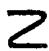
\includegraphics[keepaspectratio]{images/part001_579990b7.jpg}}

Let (C, d) be a complex. We set \(\mathbf{Z}(\mathbf{C}, d) = \operatorname{Ker}(d)\) , \(\mathbf{B}(\mathbf{C}, d) = \operatorname{Im}(d)\) ; these are graded submodules of C, called respectively the module of cycles and the module of boundaries of (C, d); the homogeneous components of \(\mathbf{Z}(\mathbf{C}, d)\) and \(\mathbf{B}(\mathbf{C}, d)\) are denoted \(\mathbf{Z}_{n}(\mathbf{C}, d) = \mathbf{Z}^{-n}(\mathbf{C}, d)\) , \(\mathbf{B}_{n}(\mathbf{C}, d) = \mathbf{B}^{-n}(\mathbf{C}, d)\) ; we have \(\mathbf{Z}_{n}(\mathbf{C}, d) = \operatorname{Ker}(d_{n})\) , \(\mathbf{B}_{n}(\mathbf{C}, d) = \operatorname{Im}(d_{n+1})\) , \(\mathbf{Z}^{n}(\mathbf{C}, d) = \operatorname{Ker}(d^{n})\) , \(\mathbf{B}^{n}(\mathbf{C}, d) = \operatorname{Im}(d^{n-1})\) .

Since \(d \circ d = 0\) , we have \(\mathrm{B}(\mathrm{C}) \subset \mathrm{Z}(\mathrm{C})\) ; two cycles are said to be homologous if their difference is a boundary; the quotient graded module \(\mathrm{H}(\mathrm{C}, d) = \mathrm{Z}(\mathrm{C}, d)/\mathrm{B}(\mathrm{C}, d)\) is called the homology module of \((\mathrm{C}, d)\) ; its elements are the homology classes; its homogeneous components are denoted \(\mathrm{H}_n(\mathrm{C}, d) = \mathrm{H}^{-n}(\mathrm{C}, d)\) .

Example. --- If C has zero differential, we have \(Z(C) = C\) , \(B(C) = 0\) and \(H(C)\) is canonically identified with \(C\) .

We have exact sequences, called canonical:

\((I_{n})\)

\[
0 \longrightarrow \mathrm{Z} _ {n} (\mathrm{C}) \longrightarrow \mathrm{C} _ {n} \stackrel {\delta_ {n}} {\longrightarrow} \mathrm{B} _ {n - 1} (\mathrm{C}) \longrightarrow 0\tag{\((\mathrm{II}_{n})\)}
\]

\[
0 \longrightarrow \mathrm{B} _ {n} (\mathrm{C}) \longrightarrow \mathrm{Z} _ {n} (\mathrm{C}) \longrightarrow \mathrm{H} _ {n} (\mathrm{C}) \longrightarrow 0
\]

\((\mathrm{III}_{n})\)

\[
0 \longrightarrow \mathrm{B} _ {n} (\mathrm{C}) \longrightarrow \mathrm{C} _ {n} \longrightarrow \mathrm{C} _ {n} / \mathrm{B} _ {n} (\mathrm{C}) \longrightarrow 0
\]

\((\mathrm{IV}_n)\)

\[
0 \longrightarrow \mathrm{H} _ {n} (\mathrm{C}) \longrightarrow \mathrm{C} _ {n} / \mathrm{B} _ {n} (\mathrm{C}) \stackrel {\overline {{\delta}} _ {n}} {\longrightarrow} \mathrm{B} _ {n - 1} (\mathrm{C}) \longrightarrow 0
\]

where \(\delta_{n}\) and \(\overline{\delta}_{n}\) are deduced from \(d_{n}\) . By combining \((\mathrm{IV}_{n})\) and \((\mathrm{II}_{n-1})\) , one obtains the exact sequence

\[
0 \rightarrow \mathrm{H} _ {n} (\mathrm{C}) \rightarrow \mathrm{C} _ {n} / \mathrm{B} _ {n} (\mathrm{C}) \rightarrow \mathrm{Z} _ {n - 1} (\mathrm{C}) \rightarrow \mathrm{H} _ {n - 1} (\mathrm{C}) \rightarrow 0,\tag{\((\mathbf{V}_n)\)}
\]

which is also written, changing n to -n

\[
0 \rightarrow \mathrm{H} ^ {n} (\mathrm{C}) \rightarrow \mathrm{C} ^ {n} / \mathrm{B} ^ {n} (\mathrm{C}) \rightarrow \mathrm{Z} ^ {n + 1} (\mathrm{C}) \rightarrow , \mathrm{H} ^ {n + 1} (\mathrm{C}) \rightarrow 0.\tag{\((\mathbf{V}^n)\)}
\]

DEFINITION 2. --- Let (C, d) and (C', d') be two complexes. A morphism \(^{1}\) from (C, d) to (C', d') is a graded A-homomorphism u of degree 0 from C to C' such that

\[
d ^ {\prime} \circ u = u \circ d.
\]

For every \(n\) we therefore have \(d_n' \circ u_n = u_{n-1} \circ d_n\) and \(d''n \circ u^n = u^{n+1} \circ d^n\) . We have

\[
u (\mathbf {Z} (\mathbf {C})) \subset \mathbf {Z} (\mathbf {C} ^ {\prime}), \quad u (\mathbf {B} (\mathbf {C})) \subset \mathbf {B} (\mathbf {C} ^ {\prime}),
\]

and we denote by \(Z(u):Z(C)\to Z(C')\) , \(B(u):B(C)\to B(C')\) , \(H(u):H(C)\to H(C')\) the homomorphisms of A-modules deduced from them; the homogeneous components of these morphisms are denoted \(Z_{n}(u)\) , \(Z^{n}(u)\) , \ldots{}

If \(v\) is another morphism of \((\mathbf{C}, d)\) to \((\mathbf{C}', d')\) , then \(u + v\) is a morphism of \((\mathbf{C}, d)\) to \((\mathbf{C}', d')\) , and we have

\[
\mathbf {Z} (u + v) = \mathbf {Z} (u) + \mathbf {Z} (v), \quad \mathbf {B} (u + v) = \mathbf {B} (u) + \mathbf {B} (v), \quad \mathbf {H} (u + v) = \mathbf {H} (u) + \mathbf {H} (v)
\]

Similarly, if A is an algebra over a commutative ring \(k\) , and if \(\lambda \in k\) , then \(\lambda u\) is a morphism of \((C, d)\) to \((C', d')\) and we have

\[
\mathbf {Z} (\lambda u) = \lambda \mathbf {Z} (u), \quad \mathbf {B} (\lambda u) = \lambda \mathbf {B} (u), \quad \mathbf {H} (\lambda u) = \lambda \mathbf {H} (u).
\]

If \(u': (C', d') \to (C'', d'')\) is another morphism of complexes, then \(u' \circ u\) is a morphism of \((C, d)\) to \((C'', d'')\) and we have

\[
\mathrm{Z} \left(u ^ {\prime} \circ u\right) = \mathrm{Z} \left(u ^ {\prime}\right) \circ \mathrm{Z} (u), \quad \mathrm{B} \left(u ^ {\prime} \circ u\right) = \mathrm{B} \left(u ^ {\prime}\right) \circ \mathrm{B} (u), \quad \mathrm{H} \left(u ^ {\prime} \circ u\right) = \mathrm{H} \left(u ^ {\prime}\right) \circ \mathrm{H} (u).
\]

It is clear that a bijective morphism is an isomorphism.

DEFINITION 3. --- Let (C, d) and (C', d') be two complexes. A homology morphism (or quasi-isomorphism) from (C, d) to (C', d') is a morphism u from (C, d) to (C', d') such that H(u) is bijective.

Every isomorphism is a homology morphism, and every morphism composed of homology morphisms is a homology morphism.

One says that (C, d) has zero homology if H(C) = 0, that is, if the unique morphism of complexes \(0 \rightarrow C\) (resp. C → 0) is a homology morphism. One says that (C, d) is acyclic in descending degree n (resp. in ascending degree n) if \(\mathrm{H}_{n}(\mathrm{C}) = 0\) (resp. \(\mathrm{H}^{n}(\mathrm{C}) = 0\) ).

Let (C, d) be a complex and \(p \in Z\) . The p-th translate of (C, d) is the complex (C(p), d(p)) obtained as follows: C(p) is the A-module obtained by shifting the grading of C by p (II, p.~163; example 3), so that

\[
\mathrm{C} (p) _ {n} = \mathrm{C} _ {n + p}, \quad \mathrm{C} (p) ^ {n} = \mathrm{C} ^ {n - p};
\]

in particular \(\mathbf{C}(p)_{0} = \mathbf{C}_{p}\) ; one also notes that C is the direct sum of its graded submodules \(\mathbf{C}_{p}(-p)\) , \(p \in \mathbf{Z}\) (resp. \(\mathbf{C}^{p}(p)\) , \(p \in \mathbf{Z}\) ). One sets \(d(p) = (-1)^{p} d\) . We have \(\mathbf{Z}(\mathbf{C}(p)) = \mathbf{Z}(\mathbf{C})(p)\) , \(\mathbf{B}(\mathbf{C}(p)) = \mathbf{B}(\mathbf{C})(p)\) and \(\mathrm{H}(\mathbf{C}(p)) = \mathrm{H}(\mathbf{C})(p)\) .

For example, \(d\) is a morphism of complexes from C to C(-1) and

\[
\mathrm{H} (d): \mathrm{H} (\mathbf {C}) \to \mathrm{H} (\mathbf {C}) (- 1)
\]

is zero.

For every morphism of complexes \(u:(\mathbf{C},d)\to(\mathbf{C}^{\prime},d^{\prime})\) , and every \(p\in\mathbf{Z}\) , \(u\) is also a morphism of \((\mathbf{C}(p),d(p))\) to \((\mathbf{C}^{\prime}(p),d^{\prime}(p))\) ; it is sometimes denoted \(u(p)\) and we have

\[
u (p) _ {n} = u _ {n + p}, \quad u (p) ^ {n} = u ^ {n - p}.
\]
